\batchmode
\documentclass[twoside]{book}

% Packages required by doxygen
\usepackage{fixltx2e}
\usepackage{calc}
\usepackage{doxygen}
\usepackage[export]{adjustbox} % also loads graphicx
\usepackage{graphicx}
\usepackage[utf8]{inputenc}
\usepackage{makeidx}
\usepackage{multicol}
\usepackage{multirow}
\PassOptionsToPackage{warn}{textcomp}
\usepackage{textcomp}
\usepackage[nointegrals]{wasysym}
\usepackage[table]{xcolor}

% Font selection
\usepackage[T1]{fontenc}
\usepackage[scaled=.90]{helvet}
\usepackage{courier}
\usepackage{amssymb}
\usepackage{sectsty}
\renewcommand{\familydefault}{\sfdefault}
\allsectionsfont{%
  \fontseries{bc}\selectfont%
  \color{darkgray}%
}
\renewcommand{\DoxyLabelFont}{%
  \fontseries{bc}\selectfont%
  \color{darkgray}%
}
\newcommand{\+}{\discretionary{\mbox{\scriptsize$\hookleftarrow$}}{}{}}

% Page & text layout
\usepackage{geometry}
\geometry{%
  a4paper,%
  top=2.5cm,%
  bottom=2.5cm,%
  left=2.5cm,%
  right=2.5cm%
}
\tolerance=750
\hfuzz=15pt
\hbadness=750
\setlength{\emergencystretch}{15pt}
\setlength{\parindent}{0cm}
\setlength{\parskip}{3ex plus 2ex minus 2ex}
\makeatletter
\renewcommand{\paragraph}{%
  \@startsection{paragraph}{4}{0ex}{-1.0ex}{1.0ex}{%
    \normalfont\normalsize\bfseries\SS@parafont%
  }%
}
\renewcommand{\subparagraph}{%
  \@startsection{subparagraph}{5}{0ex}{-1.0ex}{1.0ex}{%
    \normalfont\normalsize\bfseries\SS@subparafont%
  }%
}
\makeatother

% Headers & footers
\usepackage{fancyhdr}
\pagestyle{fancyplain}
\fancyhead[LE]{\fancyplain{}{\bfseries\thepage}}
\fancyhead[CE]{\fancyplain{}{}}
\fancyhead[RE]{\fancyplain{}{\bfseries\leftmark}}
\fancyhead[LO]{\fancyplain{}{\bfseries\rightmark}}
\fancyhead[CO]{\fancyplain{}{}}
\fancyhead[RO]{\fancyplain{}{\bfseries\thepage}}
\fancyfoot[LE]{\fancyplain{}{}}
\fancyfoot[CE]{\fancyplain{}{}}
\fancyfoot[RE]{\fancyplain{}{\bfseries\scriptsize Generated by Doxygen }}
\fancyfoot[LO]{\fancyplain{}{\bfseries\scriptsize Generated by Doxygen }}
\fancyfoot[CO]{\fancyplain{}{}}
\fancyfoot[RO]{\fancyplain{}{}}
\renewcommand{\footrulewidth}{0.4pt}
\renewcommand{\chaptermark}[1]{%
  \markboth{#1}{}%
}
\renewcommand{\sectionmark}[1]{%
  \markright{\thesection\ #1}%
}

% Indices & bibliography
\usepackage{natbib}
\usepackage[titles]{tocloft}
\setcounter{tocdepth}{3}
\setcounter{secnumdepth}{5}
\makeindex

% Hyperlinks (required, but should be loaded last)
\usepackage{ifpdf}
\ifpdf
  \usepackage[pdftex,pagebackref=true]{hyperref}
\else
  \usepackage[ps2pdf,pagebackref=true]{hyperref}
\fi
\hypersetup{%
  colorlinks=true,%
  linkcolor=blue,%
  citecolor=blue,%
  unicode%
}

% Custom commands
\newcommand{\clearemptydoublepage}{%
  \newpage{\pagestyle{empty}\cleardoublepage}%
}

\usepackage{caption}
\captionsetup{labelsep=space,justification=centering,font={bf},singlelinecheck=off,skip=4pt,position=top}

%===== C O N T E N T S =====

\begin{document}

% Titlepage & ToC
\hypersetup{pageanchor=false,
             bookmarksnumbered=true,
             pdfencoding=unicode
            }
\pagenumbering{alph}
\pagenumbering{arabic}
\hypersetup{pageanchor=true}

%--- Begin generated contents ---
\chapter{Demo problem\+: A one-\/dimensional eigenproblem with complex eigenvalues}
\label{index}\hypertarget{index}{}\hypertarget{index_q}{}\section{A few quick questions...}\label{index_q}
Since {\ttfamily oomph-\/lib} is developed as open-\/source software, any evidence that the code is being downloaded and used is very helpful for us as it helps to justify our continued work on this project.

We would therefore be extremely grateful if you could provide the information requested in the form below. Pressing the \char`\"{}submit\char`\"{} button will get you to the actual download page.

{\bfseries Note\+:} 
\begin{DoxyItemize}
\item All information will be treated as confidential. 
\item If you provide your email address and check the appropriate box we will add you to our mailing list to inform you of upgrades and bug fixes to the code. Rest assured that the mailing list is {\bfseries very low volume} -- we have better things to do than to bombard you with email. 
\item If you still feel reluctant to provide any of the information requested, feel free to enter some dummy input. The form will check that {\bfseries some} information has been entered but entering your name as \char`\"{}\+Joe Cool\char`\"{} is perfectly acceptable -- this is to discourage people from not providing the information simply because they are too lazy to type... 
\end{DoxyItemize}



 







 

 \hypertarget{index_pdf}{}\section{P\+D\+F file}\label{index_pdf}
A \href{../latex/refman.pdf}{\tt pdf version} of this document is available. \end{document}

\chapter{Namespace Index}
\section{Namespace List}
Here is a list of all namespaces with brief descriptions\+:\begin{DoxyCompactList}
\item\contentsline{section}{\hyperlink{namespaceGlobal__Physical__Variables}{Global\+\_\+\+Physical\+\_\+\+Variables} \\*Global variables that represent physical properties }{\pageref{namespaceGlobal__Physical__Variables}}{}
\item\contentsline{section}{\hyperlink{namespaceoomph}{oomph} }{\pageref{namespaceoomph}}{}
\item\contentsline{section}{\hyperlink{namespacePhysical__Variables}{Physical\+\_\+\+Variables} \\*Namespace for the solution of 2D linear shell equation }{\pageref{namespacePhysical__Variables}}{}
\end{DoxyCompactList}

\chapter{Hierarchical Index}
\section{Class Hierarchy}
This inheritance list is sorted roughly, but not completely, alphabetically\+:\begin{DoxyCompactList}
\item Problem\begin{DoxyCompactList}
\item \contentsline{section}{Unstructured\+Solid\+Problem$<$ E\+L\+E\+M\+E\+NT $>$}{\pageref{classUnstructuredSolidProblem}}{}
\end{DoxyCompactList}
\end{DoxyCompactList}

\chapter{Class Index}
\section{Class List}
Here are the classes, structs, unions and interfaces with brief descriptions\+:\begin{DoxyCompactList}
\item\contentsline{section}{\hyperlink{classPMLProblem}{P\+M\+L\+Problem$<$ E\+L\+E\+M\+E\+N\+T $>$} }{\pageref{classPMLProblem}}{}
\item\contentsline{section}{\hyperlink{classGlobalParameters_1_1TestPMLMapping}{Global\+Parameters\+::\+Test\+P\+M\+L\+Mapping} }{\pageref{classGlobalParameters_1_1TestPMLMapping}}{}
\end{DoxyCompactList}

\chapter{File Index}
\section{File List}
Here is a list of all files with brief descriptions\+:\begin{DoxyCompactList}
\item\contentsline{section}{\hyperlink{jeffery__orbit_8cc}{jeffery\+\_\+orbit.\+cc} }{\pageref{jeffery__orbit_8cc}}{}
\item\contentsline{section}{\hyperlink{jeffery__orbit_8txt__doxygenified_8h}{jeffery\+\_\+orbit.\+txt\+\_\+doxygenified.\+h} }{\pageref{jeffery__orbit_8txt__doxygenified_8h}}{}
\item\contentsline{section}{\hyperlink{my__taylor__hood__elements_8h}{my\+\_\+taylor\+\_\+hood\+\_\+elements.\+h} }{\pageref{my__taylor__hood__elements_8h}}{}
\end{DoxyCompactList}

\chapter{Namespace Documentation}
\hypertarget{namespaceEigenproblemShift}{}\section{Eigenproblem\+Shift Namespace Reference}
\label{namespaceEigenproblemShift}\index{Eigenproblem\+Shift@{Eigenproblem\+Shift}}


Namespace for the shift applied to the eigenproblem.  


\subsection*{Variables}
\begin{DoxyCompactItemize}
\item 
double \hyperlink{namespaceEigenproblemShift_a82e816b5ecba937123c65c5bd953a2fb}{Mu} = 6.\+5
\end{DoxyCompactItemize}


\subsection{Detailed Description}
Namespace for the shift applied to the eigenproblem. 

\subsection{Variable Documentation}
\mbox{\Hypertarget{namespaceEigenproblemShift_a82e816b5ecba937123c65c5bd953a2fb}\label{namespaceEigenproblemShift_a82e816b5ecba937123c65c5bd953a2fb}} 
\index{Eigenproblem\+Shift@{Eigenproblem\+Shift}!Mu@{Mu}}
\index{Mu@{Mu}!Eigenproblem\+Shift@{Eigenproblem\+Shift}}
\subsubsection{\texorpdfstring{Mu}{Mu}}
{\footnotesize\ttfamily double Eigenproblem\+Shift\+::\+Mu = 6.\+5}



Definition at line 50 of file complex\+\_\+harmonic.\+cc.



Referenced by Complex\+Harmonic\+Equations\+::fill\+\_\+in\+\_\+contribution\+\_\+to\+\_\+jacobian\+\_\+and\+\_\+mass\+\_\+matrix().


\chapter{Class Documentation}
\hypertarget{classComplexHarmonicEquations}{}\section{Complex\+Harmonic\+Equations Class Reference}
\label{classComplexHarmonicEquations}\index{Complex\+Harmonic\+Equations@{Complex\+Harmonic\+Equations}}
Inheritance diagram for Complex\+Harmonic\+Equations\+:\begin{figure}[H]
\begin{center}
\leavevmode
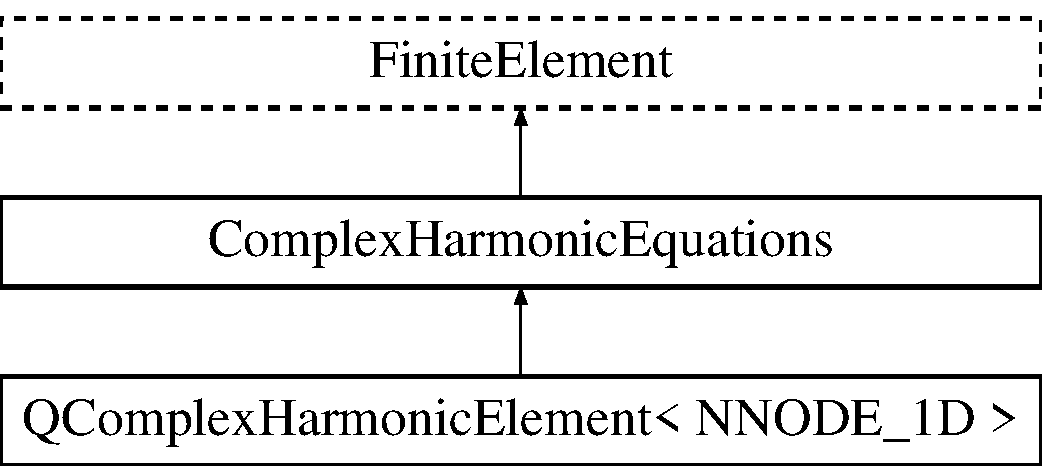
\includegraphics[height=3.000000cm]{classComplexHarmonicEquations}
\end{center}
\end{figure}
\subsection*{Public Member Functions}
\begin{DoxyCompactItemize}
\item 
\hyperlink{classComplexHarmonicEquations_aa93feb265f731b0d82c3c1c4c29f183d}{Complex\+Harmonic\+Equations} ()
\begin{DoxyCompactList}\small\item\em Empty Constructor. \end{DoxyCompactList}\item 
virtual double \hyperlink{classComplexHarmonicEquations_af4ff638cb40e23c3574631423fd56bce}{u} (const unsigned \&n) const
\begin{DoxyCompactList}\small\item\em Access function\+: First eigenfunction value at local node n Note that solving the eigenproblem does not assign values to this storage space. It is used for output purposes only. \end{DoxyCompactList}\item 
virtual double \hyperlink{classComplexHarmonicEquations_a9b3955ee987827d831e44eeb43dcae63}{w} (const unsigned \&n) const
\begin{DoxyCompactList}\small\item\em Second eigenfunction value at local node n. \end{DoxyCompactList}\item 
void \hyperlink{classComplexHarmonicEquations_a9185e07b984e735c1c45b6f5a6c02b5f}{output} (ostream \&outfile)
\begin{DoxyCompactList}\small\item\em Output the eigenfunction with default number of plot points. \end{DoxyCompactList}\item 
void \hyperlink{classComplexHarmonicEquations_a141e0a24096323472fcd10138b6fd5fa}{output} (ostream \&outfile, const unsigned \&nplot)
\begin{DoxyCompactList}\small\item\em Output FE representation of soln\+: x,y,u or x,y,z,u at Nplot plot points. \end{DoxyCompactList}\item 
void \hyperlink{classComplexHarmonicEquations_a4c67a0c220f61d6c300703f29c00b1ef}{fill\+\_\+in\+\_\+contribution\+\_\+to\+\_\+jacobian\+\_\+and\+\_\+mass\+\_\+matrix} (Vector$<$ double $>$ \&residuals, Dense\+Matrix$<$ double $>$ \&jacobian, Dense\+Matrix$<$ double $>$ \&mass\+\_\+matrix)
\begin{DoxyCompactList}\small\item\em Assemble the contributions to the jacobian and mass matrices. \end{DoxyCompactList}\item 
double \hyperlink{classComplexHarmonicEquations_a9e8774f4cf492bd267c0a170bf4f81a6}{interpolated\+\_\+u} (const Vector$<$ double $>$ \&s) const
\begin{DoxyCompactList}\small\item\em Return FE representation of function value u(s) at local coordinate s. \end{DoxyCompactList}\item 
double \hyperlink{classComplexHarmonicEquations_a73b34acf2038ae9c2ef3f3e61d9c1cd7}{interpolated\+\_\+w} (const Vector$<$ double $>$ \&s) const
\begin{DoxyCompactList}\small\item\em Return FE representation of function value w(s) at local coordinate s. \end{DoxyCompactList}\end{DoxyCompactItemize}
\subsection*{Protected Member Functions}
\begin{DoxyCompactItemize}
\item 
virtual double \hyperlink{classComplexHarmonicEquations_a59048c598e2fba3e11aa5985ffaf4d76}{dshape\+\_\+eulerian} (const Vector$<$ double $>$ \&s, Shape \&psi, D\+Shape \&dpsidx) const =0
\begin{DoxyCompactList}\small\item\em Shape/test functions and derivs w.\+r.\+t. to global coords at local coord. s; return Jacobian of mapping. \end{DoxyCompactList}\item 
virtual double \hyperlink{classComplexHarmonicEquations_a60c71828f2d4c1c2363dcb1d1f334fff}{dshape\+\_\+eulerian\+\_\+at\+\_\+knot} (const unsigned \&ipt, Shape \&psi, D\+Shape \&dpsidx) const =0
\begin{DoxyCompactList}\small\item\em Shape/test functions and derivs w.\+r.\+t. to global coords at integration point ipt; return Jacobian of mapping. \end{DoxyCompactList}\item 
virtual int \hyperlink{classComplexHarmonicEquations_a3538cae061c24db2db1fc277c0a09da4}{u\+\_\+local\+\_\+eqn} (const unsigned \&n, const unsigned \&i)
\begin{DoxyCompactList}\small\item\em Access function that returns the local equation number of the unknown in the problem. Default is to assume that it is the first (only) value stored at the node. \end{DoxyCompactList}\end{DoxyCompactItemize}


\subsection{Detailed Description}
A class for all elements that solve the eigenvalue problem \[ \frac{\partial w}{\partial x} = \lambda u \] \[ \frac{\partial u}{\partial x} = (\lambda - \mu) w \] This class contains the generic maths. Shape functions, geometric mapping etc. must get implemented in derived class. 

Definition at line 92 of file complex\+\_\+harmonic.\+cc.



\subsection{Constructor \& Destructor Documentation}
\mbox{\Hypertarget{classComplexHarmonicEquations_aa93feb265f731b0d82c3c1c4c29f183d}\label{classComplexHarmonicEquations_aa93feb265f731b0d82c3c1c4c29f183d}} 
\index{Complex\+Harmonic\+Equations@{Complex\+Harmonic\+Equations}!Complex\+Harmonic\+Equations@{Complex\+Harmonic\+Equations}}
\index{Complex\+Harmonic\+Equations@{Complex\+Harmonic\+Equations}!Complex\+Harmonic\+Equations@{Complex\+Harmonic\+Equations}}
\subsubsection{\texorpdfstring{Complex\+Harmonic\+Equations()}{ComplexHarmonicEquations()}}
{\footnotesize\ttfamily Complex\+Harmonic\+Equations\+::\+Complex\+Harmonic\+Equations (\begin{DoxyParamCaption}{ }\end{DoxyParamCaption})\hspace{0.3cm}{\ttfamily [inline]}}



Empty Constructor. 



Definition at line 97 of file complex\+\_\+harmonic.\+cc.



\subsection{Member Function Documentation}
\mbox{\Hypertarget{classComplexHarmonicEquations_a59048c598e2fba3e11aa5985ffaf4d76}\label{classComplexHarmonicEquations_a59048c598e2fba3e11aa5985ffaf4d76}} 
\index{Complex\+Harmonic\+Equations@{Complex\+Harmonic\+Equations}!dshape\+\_\+eulerian@{dshape\+\_\+eulerian}}
\index{dshape\+\_\+eulerian@{dshape\+\_\+eulerian}!Complex\+Harmonic\+Equations@{Complex\+Harmonic\+Equations}}
\subsubsection{\texorpdfstring{dshape\+\_\+eulerian()}{dshape\_eulerian()}}
{\footnotesize\ttfamily virtual double Complex\+Harmonic\+Equations\+::dshape\+\_\+eulerian (\begin{DoxyParamCaption}\item[{const Vector$<$ double $>$ \&}]{s,  }\item[{Shape \&}]{psi,  }\item[{D\+Shape \&}]{dpsidx }\end{DoxyParamCaption}) const\hspace{0.3cm}{\ttfamily [protected]}, {\ttfamily [pure virtual]}}



Shape/test functions and derivs w.\+r.\+t. to global coords at local coord. s; return Jacobian of mapping. 



Implemented in \hyperlink{classQComplexHarmonicElement_a7c97d4e8c5433a44640d30c936d69ffb}{Q\+Complex\+Harmonic\+Element$<$ N\+N\+O\+D\+E\+\_\+1\+D $>$}.

\mbox{\Hypertarget{classComplexHarmonicEquations_a60c71828f2d4c1c2363dcb1d1f334fff}\label{classComplexHarmonicEquations_a60c71828f2d4c1c2363dcb1d1f334fff}} 
\index{Complex\+Harmonic\+Equations@{Complex\+Harmonic\+Equations}!dshape\+\_\+eulerian\+\_\+at\+\_\+knot@{dshape\+\_\+eulerian\+\_\+at\+\_\+knot}}
\index{dshape\+\_\+eulerian\+\_\+at\+\_\+knot@{dshape\+\_\+eulerian\+\_\+at\+\_\+knot}!Complex\+Harmonic\+Equations@{Complex\+Harmonic\+Equations}}
\subsubsection{\texorpdfstring{dshape\+\_\+eulerian\+\_\+at\+\_\+knot()}{dshape\_eulerian\_at\_knot()}}
{\footnotesize\ttfamily virtual double Complex\+Harmonic\+Equations\+::dshape\+\_\+eulerian\+\_\+at\+\_\+knot (\begin{DoxyParamCaption}\item[{const unsigned \&}]{ipt,  }\item[{Shape \&}]{psi,  }\item[{D\+Shape \&}]{dpsidx }\end{DoxyParamCaption}) const\hspace{0.3cm}{\ttfamily [protected]}, {\ttfamily [pure virtual]}}



Shape/test functions and derivs w.\+r.\+t. to global coords at integration point ipt; return Jacobian of mapping. 



Implemented in \hyperlink{classQComplexHarmonicElement_a3f8d1d9396135d4d86f416dcf6c23904}{Q\+Complex\+Harmonic\+Element$<$ N\+N\+O\+D\+E\+\_\+1\+D $>$}.

\mbox{\Hypertarget{classComplexHarmonicEquations_a4c67a0c220f61d6c300703f29c00b1ef}\label{classComplexHarmonicEquations_a4c67a0c220f61d6c300703f29c00b1ef}} 
\index{Complex\+Harmonic\+Equations@{Complex\+Harmonic\+Equations}!fill\+\_\+in\+\_\+contribution\+\_\+to\+\_\+jacobian\+\_\+and\+\_\+mass\+\_\+matrix@{fill\+\_\+in\+\_\+contribution\+\_\+to\+\_\+jacobian\+\_\+and\+\_\+mass\+\_\+matrix}}
\index{fill\+\_\+in\+\_\+contribution\+\_\+to\+\_\+jacobian\+\_\+and\+\_\+mass\+\_\+matrix@{fill\+\_\+in\+\_\+contribution\+\_\+to\+\_\+jacobian\+\_\+and\+\_\+mass\+\_\+matrix}!Complex\+Harmonic\+Equations@{Complex\+Harmonic\+Equations}}
\subsubsection{\texorpdfstring{fill\+\_\+in\+\_\+contribution\+\_\+to\+\_\+jacobian\+\_\+and\+\_\+mass\+\_\+matrix()}{fill\_in\_contribution\_to\_jacobian\_and\_mass\_matrix()}}
{\footnotesize\ttfamily void Complex\+Harmonic\+Equations\+::fill\+\_\+in\+\_\+contribution\+\_\+to\+\_\+jacobian\+\_\+and\+\_\+mass\+\_\+matrix (\begin{DoxyParamCaption}\item[{Vector$<$ double $>$ \&}]{residuals,  }\item[{Dense\+Matrix$<$ double $>$ \&}]{jacobian,  }\item[{Dense\+Matrix$<$ double $>$ \&}]{mass\+\_\+matrix }\end{DoxyParamCaption})\hspace{0.3cm}{\ttfamily [inline]}}



Assemble the contributions to the jacobian and mass matrices. 



Definition at line 142 of file complex\+\_\+harmonic.\+cc.



References Eigenproblem\+Shift\+::\+Mu.

\mbox{\Hypertarget{classComplexHarmonicEquations_a9e8774f4cf492bd267c0a170bf4f81a6}\label{classComplexHarmonicEquations_a9e8774f4cf492bd267c0a170bf4f81a6}} 
\index{Complex\+Harmonic\+Equations@{Complex\+Harmonic\+Equations}!interpolated\+\_\+u@{interpolated\+\_\+u}}
\index{interpolated\+\_\+u@{interpolated\+\_\+u}!Complex\+Harmonic\+Equations@{Complex\+Harmonic\+Equations}}
\subsubsection{\texorpdfstring{interpolated\+\_\+u()}{interpolated\_u()}}
{\footnotesize\ttfamily double Complex\+Harmonic\+Equations\+::interpolated\+\_\+u (\begin{DoxyParamCaption}\item[{const Vector$<$ double $>$ \&}]{s }\end{DoxyParamCaption}) const\hspace{0.3cm}{\ttfamily [inline]}}



Return FE representation of function value u(s) at local coordinate s. 



Definition at line 232 of file complex\+\_\+harmonic.\+cc.

\mbox{\Hypertarget{classComplexHarmonicEquations_a73b34acf2038ae9c2ef3f3e61d9c1cd7}\label{classComplexHarmonicEquations_a73b34acf2038ae9c2ef3f3e61d9c1cd7}} 
\index{Complex\+Harmonic\+Equations@{Complex\+Harmonic\+Equations}!interpolated\+\_\+w@{interpolated\+\_\+w}}
\index{interpolated\+\_\+w@{interpolated\+\_\+w}!Complex\+Harmonic\+Equations@{Complex\+Harmonic\+Equations}}
\subsubsection{\texorpdfstring{interpolated\+\_\+w()}{interpolated\_w()}}
{\footnotesize\ttfamily double Complex\+Harmonic\+Equations\+::interpolated\+\_\+w (\begin{DoxyParamCaption}\item[{const Vector$<$ double $>$ \&}]{s }\end{DoxyParamCaption}) const\hspace{0.3cm}{\ttfamily [inline]}}



Return FE representation of function value w(s) at local coordinate s. 



Definition at line 253 of file complex\+\_\+harmonic.\+cc.

\mbox{\Hypertarget{classComplexHarmonicEquations_a9185e07b984e735c1c45b6f5a6c02b5f}\label{classComplexHarmonicEquations_a9185e07b984e735c1c45b6f5a6c02b5f}} 
\index{Complex\+Harmonic\+Equations@{Complex\+Harmonic\+Equations}!output@{output}}
\index{output@{output}!Complex\+Harmonic\+Equations@{Complex\+Harmonic\+Equations}}
\subsubsection{\texorpdfstring{output()}{output()}\hspace{0.1cm}{\footnotesize\ttfamily [1/2]}}
{\footnotesize\ttfamily void Complex\+Harmonic\+Equations\+::output (\begin{DoxyParamCaption}\item[{ostream \&}]{outfile }\end{DoxyParamCaption})\hspace{0.3cm}{\ttfamily [inline]}}



Output the eigenfunction with default number of plot points. 



Definition at line 110 of file complex\+\_\+harmonic.\+cc.



Referenced by Q\+Complex\+Harmonic\+Element$<$ N\+N\+O\+D\+E\+\_\+1\+D $>$\+::output().

\mbox{\Hypertarget{classComplexHarmonicEquations_a141e0a24096323472fcd10138b6fd5fa}\label{classComplexHarmonicEquations_a141e0a24096323472fcd10138b6fd5fa}} 
\index{Complex\+Harmonic\+Equations@{Complex\+Harmonic\+Equations}!output@{output}}
\index{output@{output}!Complex\+Harmonic\+Equations@{Complex\+Harmonic\+Equations}}
\subsubsection{\texorpdfstring{output()}{output()}\hspace{0.1cm}{\footnotesize\ttfamily [2/2]}}
{\footnotesize\ttfamily void Complex\+Harmonic\+Equations\+::output (\begin{DoxyParamCaption}\item[{ostream \&}]{outfile,  }\item[{const unsigned \&}]{nplot }\end{DoxyParamCaption})\hspace{0.3cm}{\ttfamily [inline]}}



Output FE representation of soln\+: x,y,u or x,y,z,u at Nplot plot points. 



Definition at line 118 of file complex\+\_\+harmonic.\+cc.

\mbox{\Hypertarget{classComplexHarmonicEquations_af4ff638cb40e23c3574631423fd56bce}\label{classComplexHarmonicEquations_af4ff638cb40e23c3574631423fd56bce}} 
\index{Complex\+Harmonic\+Equations@{Complex\+Harmonic\+Equations}!u@{u}}
\index{u@{u}!Complex\+Harmonic\+Equations@{Complex\+Harmonic\+Equations}}
\subsubsection{\texorpdfstring{u()}{u()}}
{\footnotesize\ttfamily virtual double Complex\+Harmonic\+Equations\+::u (\begin{DoxyParamCaption}\item[{const unsigned \&}]{n }\end{DoxyParamCaption}) const\hspace{0.3cm}{\ttfamily [inline]}, {\ttfamily [virtual]}}



Access function\+: First eigenfunction value at local node n Note that solving the eigenproblem does not assign values to this storage space. It is used for output purposes only. 



Definition at line 102 of file complex\+\_\+harmonic.\+cc.

\mbox{\Hypertarget{classComplexHarmonicEquations_a3538cae061c24db2db1fc277c0a09da4}\label{classComplexHarmonicEquations_a3538cae061c24db2db1fc277c0a09da4}} 
\index{Complex\+Harmonic\+Equations@{Complex\+Harmonic\+Equations}!u\+\_\+local\+\_\+eqn@{u\+\_\+local\+\_\+eqn}}
\index{u\+\_\+local\+\_\+eqn@{u\+\_\+local\+\_\+eqn}!Complex\+Harmonic\+Equations@{Complex\+Harmonic\+Equations}}
\subsubsection{\texorpdfstring{u\+\_\+local\+\_\+eqn()}{u\_local\_eqn()}}
{\footnotesize\ttfamily virtual int Complex\+Harmonic\+Equations\+::u\+\_\+local\+\_\+eqn (\begin{DoxyParamCaption}\item[{const unsigned \&}]{n,  }\item[{const unsigned \&}]{i }\end{DoxyParamCaption})\hspace{0.3cm}{\ttfamily [inline]}, {\ttfamily [protected]}, {\ttfamily [virtual]}}



Access function that returns the local equation number of the unknown in the problem. Default is to assume that it is the first (only) value stored at the node. 



Definition at line 291 of file complex\+\_\+harmonic.\+cc.

\mbox{\Hypertarget{classComplexHarmonicEquations_a9b3955ee987827d831e44eeb43dcae63}\label{classComplexHarmonicEquations_a9b3955ee987827d831e44eeb43dcae63}} 
\index{Complex\+Harmonic\+Equations@{Complex\+Harmonic\+Equations}!w@{w}}
\index{w@{w}!Complex\+Harmonic\+Equations@{Complex\+Harmonic\+Equations}}
\subsubsection{\texorpdfstring{w()}{w()}}
{\footnotesize\ttfamily virtual double Complex\+Harmonic\+Equations\+::w (\begin{DoxyParamCaption}\item[{const unsigned \&}]{n }\end{DoxyParamCaption}) const\hspace{0.3cm}{\ttfamily [inline]}, {\ttfamily [virtual]}}



Second eigenfunction value at local node n. 



Definition at line 106 of file complex\+\_\+harmonic.\+cc.



The documentation for this class was generated from the following file\+:\begin{DoxyCompactItemize}
\item 
\hyperlink{complex__harmonic_8cc}{complex\+\_\+harmonic.\+cc}\end{DoxyCompactItemize}

\hypertarget{classComplexHarmonicProblem}{}\section{Complex\+Harmonic\+Problem$<$ E\+L\+E\+M\+E\+NT, E\+I\+G\+E\+N\+\_\+\+S\+O\+L\+V\+ER $>$ Class Template Reference}
\label{classComplexHarmonicProblem}\index{Complex\+Harmonic\+Problem$<$ E\+L\+E\+M\+E\+N\+T, E\+I\+G\+E\+N\+\_\+\+S\+O\+L\+V\+E\+R $>$@{Complex\+Harmonic\+Problem$<$ E\+L\+E\+M\+E\+N\+T, E\+I\+G\+E\+N\+\_\+\+S\+O\+L\+V\+E\+R $>$}}


1D Complex\+Harmonic problem in unit interval.  


Inheritance diagram for Complex\+Harmonic\+Problem$<$ E\+L\+E\+M\+E\+NT, E\+I\+G\+E\+N\+\_\+\+S\+O\+L\+V\+ER $>$\+:\begin{figure}[H]
\begin{center}
\leavevmode
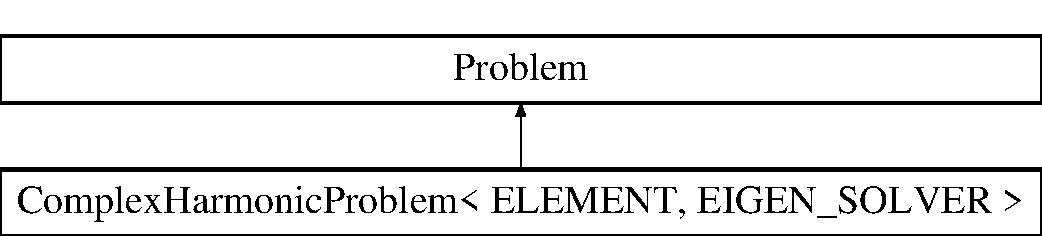
\includegraphics[height=2.000000cm]{classComplexHarmonicProblem}
\end{center}
\end{figure}
\subsection*{Public Member Functions}
\begin{DoxyCompactItemize}
\item 
\hyperlink{classComplexHarmonicProblem_aaec243aef8d954804e203f5d310b0800}{Complex\+Harmonic\+Problem} (const unsigned \&n\+\_\+element)
\begin{DoxyCompactList}\small\item\em Constructor\+: Pass number of elements and pointer to source function. \end{DoxyCompactList}\item 
\hyperlink{classComplexHarmonicProblem_a2222e80aab2660c62cbf01c5bba842fa}{$\sim$\+Complex\+Harmonic\+Problem} ()
\begin{DoxyCompactList}\small\item\em Destructor. Clean up the mesh and solver. \end{DoxyCompactList}\item 
void \hyperlink{classComplexHarmonicProblem_a3453c3c11a76fbab8c6383b52b6b33d7}{solve} (const unsigned \&label)
\begin{DoxyCompactList}\small\item\em Solve the problem. \end{DoxyCompactList}\item 
void \hyperlink{classComplexHarmonicProblem_a984616c738c9bc14a93ad825a87b0051}{doc\+\_\+solution} (const unsigned \&label)
\begin{DoxyCompactList}\small\item\em Doc the solution, pass the number of the case considered, so that output files can be distinguished. \end{DoxyCompactList}\end{DoxyCompactItemize}


\subsection{Detailed Description}
\subsubsection*{template$<$class E\+L\+E\+M\+E\+NT, class E\+I\+G\+E\+N\+\_\+\+S\+O\+L\+V\+ER$>$\newline
class Complex\+Harmonic\+Problem$<$ E\+L\+E\+M\+E\+N\+T, E\+I\+G\+E\+N\+\_\+\+S\+O\+L\+V\+E\+R $>$}

1D Complex\+Harmonic problem in unit interval. 

Definition at line 353 of file complex\+\_\+harmonic.\+cc.



\subsection{Constructor \& Destructor Documentation}
\mbox{\Hypertarget{classComplexHarmonicProblem_aaec243aef8d954804e203f5d310b0800}\label{classComplexHarmonicProblem_aaec243aef8d954804e203f5d310b0800}} 
\index{Complex\+Harmonic\+Problem@{Complex\+Harmonic\+Problem}!Complex\+Harmonic\+Problem@{Complex\+Harmonic\+Problem}}
\index{Complex\+Harmonic\+Problem@{Complex\+Harmonic\+Problem}!Complex\+Harmonic\+Problem@{Complex\+Harmonic\+Problem}}
\subsubsection{\texorpdfstring{Complex\+Harmonic\+Problem()}{ComplexHarmonicProblem()}}
{\footnotesize\ttfamily template$<$class E\+L\+E\+M\+E\+NT , class E\+I\+G\+E\+N\+\_\+\+S\+O\+L\+V\+ER $>$ \\
\hyperlink{classComplexHarmonicProblem}{Complex\+Harmonic\+Problem}$<$ E\+L\+E\+M\+E\+NT, E\+I\+G\+E\+N\+\_\+\+S\+O\+L\+V\+ER $>$\+::\hyperlink{classComplexHarmonicProblem}{Complex\+Harmonic\+Problem} (\begin{DoxyParamCaption}\item[{const unsigned \&}]{n\+\_\+element }\end{DoxyParamCaption})}



Constructor\+: Pass number of elements and pointer to source function. 

Constructor for 1D Complex\+Harmonic problem in unit interval. Discretise the 1D domain with n\+\_\+element elements of type E\+L\+E\+M\+E\+NT. Specify function pointer to source function. 

Definition at line 381 of file complex\+\_\+harmonic.\+cc.

\mbox{\Hypertarget{classComplexHarmonicProblem_a2222e80aab2660c62cbf01c5bba842fa}\label{classComplexHarmonicProblem_a2222e80aab2660c62cbf01c5bba842fa}} 
\index{Complex\+Harmonic\+Problem@{Complex\+Harmonic\+Problem}!````~Complex\+Harmonic\+Problem@{$\sim$\+Complex\+Harmonic\+Problem}}
\index{````~Complex\+Harmonic\+Problem@{$\sim$\+Complex\+Harmonic\+Problem}!Complex\+Harmonic\+Problem@{Complex\+Harmonic\+Problem}}
\subsubsection{\texorpdfstring{$\sim$\+Complex\+Harmonic\+Problem()}{~ComplexHarmonicProblem()}}
{\footnotesize\ttfamily template$<$class E\+L\+E\+M\+E\+NT, class E\+I\+G\+E\+N\+\_\+\+S\+O\+L\+V\+ER$>$ \\
\hyperlink{classComplexHarmonicProblem}{Complex\+Harmonic\+Problem}$<$ E\+L\+E\+M\+E\+NT, E\+I\+G\+E\+N\+\_\+\+S\+O\+L\+V\+ER $>$\+::$\sim$\hyperlink{classComplexHarmonicProblem}{Complex\+Harmonic\+Problem} (\begin{DoxyParamCaption}{ }\end{DoxyParamCaption})\hspace{0.3cm}{\ttfamily [inline]}}



Destructor. Clean up the mesh and solver. 



Definition at line 361 of file complex\+\_\+harmonic.\+cc.



\subsection{Member Function Documentation}
\mbox{\Hypertarget{classComplexHarmonicProblem_a984616c738c9bc14a93ad825a87b0051}\label{classComplexHarmonicProblem_a984616c738c9bc14a93ad825a87b0051}} 
\index{Complex\+Harmonic\+Problem@{Complex\+Harmonic\+Problem}!doc\+\_\+solution@{doc\+\_\+solution}}
\index{doc\+\_\+solution@{doc\+\_\+solution}!Complex\+Harmonic\+Problem@{Complex\+Harmonic\+Problem}}
\subsubsection{\texorpdfstring{doc\+\_\+solution()}{doc\_solution()}}
{\footnotesize\ttfamily template$<$class E\+L\+E\+M\+E\+NT , class E\+I\+G\+E\+N\+\_\+\+S\+O\+L\+V\+ER $>$ \\
void \hyperlink{classComplexHarmonicProblem}{Complex\+Harmonic\+Problem}$<$ E\+L\+E\+M\+E\+NT, E\+I\+G\+E\+N\+\_\+\+S\+O\+L\+V\+ER $>$\+::doc\+\_\+solution (\begin{DoxyParamCaption}\item[{const unsigned \&}]{label }\end{DoxyParamCaption})}



Doc the solution, pass the number of the case considered, so that output files can be distinguished. 

Doc the solution in tecplot format. Label files with label. 

Definition at line 420 of file complex\+\_\+harmonic.\+cc.



References Complex\+Harmonic\+Problem$<$ E\+L\+E\+M\+E\+N\+T, E\+I\+G\+E\+N\+\_\+\+S\+O\+L\+V\+E\+R $>$\+::solve().

\mbox{\Hypertarget{classComplexHarmonicProblem_a3453c3c11a76fbab8c6383b52b6b33d7}\label{classComplexHarmonicProblem_a3453c3c11a76fbab8c6383b52b6b33d7}} 
\index{Complex\+Harmonic\+Problem@{Complex\+Harmonic\+Problem}!solve@{solve}}
\index{solve@{solve}!Complex\+Harmonic\+Problem@{Complex\+Harmonic\+Problem}}
\subsubsection{\texorpdfstring{solve()}{solve()}}
{\footnotesize\ttfamily template$<$class E\+L\+E\+M\+E\+NT , class E\+I\+G\+E\+N\+\_\+\+S\+O\+L\+V\+ER $>$ \\
void \hyperlink{classComplexHarmonicProblem}{Complex\+Harmonic\+Problem}$<$ E\+L\+E\+M\+E\+NT, E\+I\+G\+E\+N\+\_\+\+S\+O\+L\+V\+ER $>$\+::solve (\begin{DoxyParamCaption}\item[{const unsigned \&}]{label }\end{DoxyParamCaption})}



Solve the problem. 

Solve the eigenproblem. 

Definition at line 444 of file complex\+\_\+harmonic.\+cc.



Referenced by Complex\+Harmonic\+Problem$<$ E\+L\+E\+M\+E\+N\+T, E\+I\+G\+E\+N\+\_\+\+S\+O\+L\+V\+E\+R $>$\+::doc\+\_\+solution(), and main().



The documentation for this class was generated from the following file\+:\begin{DoxyCompactItemize}
\item 
\hyperlink{complex__harmonic_8cc}{complex\+\_\+harmonic.\+cc}\end{DoxyCompactItemize}

\hypertarget{classComplexLess}{}\section{Complex\+Less$<$ T $>$ Class Template Reference}
\label{classComplexLess}\index{Complex\+Less$<$ T $>$@{Complex\+Less$<$ T $>$}}
\subsection*{Public Member Functions}
\begin{DoxyCompactItemize}
\item 
bool \hyperlink{classComplexLess_abb81bdb8dd1f9076863b5f3523272343}{operator()} (const complex$<$ T $>$ \&x, const complex$<$ T $>$ \&y) const
\begin{DoxyCompactList}\small\item\em Comparison in terms of magnitude of complex number. \end{DoxyCompactList}\item 
bool \hyperlink{classComplexLess_abb81bdb8dd1f9076863b5f3523272343}{operator()} (const complex$<$ T $>$ \&x, const complex$<$ T $>$ \&y) const
\begin{DoxyCompactList}\small\item\em Comparison. Are the values identical or not? \end{DoxyCompactList}\end{DoxyCompactItemize}


\subsection{Detailed Description}
\subsubsection*{template$<$class T$>$\newline
class Complex\+Less$<$ T $>$}

Function-\/type-\/object to perform comparison of complex data types Needed to sort the complex eigenvalues into order based on the size of the real part. 

Definition at line 60 of file complex\+\_\+harmonic.\+cc.



\subsection{Member Function Documentation}
\mbox{\Hypertarget{classComplexLess_abb81bdb8dd1f9076863b5f3523272343}\label{classComplexLess_abb81bdb8dd1f9076863b5f3523272343}} 
\index{Complex\+Less@{Complex\+Less}!operator()@{operator()}}
\index{operator()@{operator()}!Complex\+Less@{Complex\+Less}}
\subsubsection{\texorpdfstring{operator()()}{operator()()}\hspace{0.1cm}{\footnotesize\ttfamily [1/2]}}
{\footnotesize\ttfamily template$<$class T $>$ \\
bool \hyperlink{classComplexLess}{Complex\+Less}$<$ T $>$\+::operator() (\begin{DoxyParamCaption}\item[{const complex$<$ T $>$ \&}]{x,  }\item[{const complex$<$ T $>$ \&}]{y }\end{DoxyParamCaption}) const\hspace{0.3cm}{\ttfamily [inline]}}



Comparison. Are the values identical or not? 



Definition at line 55 of file harmonic.\+cc.

\mbox{\Hypertarget{classComplexLess_abb81bdb8dd1f9076863b5f3523272343}\label{classComplexLess_abb81bdb8dd1f9076863b5f3523272343}} 
\index{Complex\+Less@{Complex\+Less}!operator()@{operator()}}
\index{operator()@{operator()}!Complex\+Less@{Complex\+Less}}
\subsubsection{\texorpdfstring{operator()()}{operator()()}\hspace{0.1cm}{\footnotesize\ttfamily [2/2]}}
{\footnotesize\ttfamily template$<$class T $>$ \\
bool \hyperlink{classComplexLess}{Complex\+Less}$<$ T $>$\+::operator() (\begin{DoxyParamCaption}\item[{const complex$<$ T $>$ \&}]{x,  }\item[{const complex$<$ T $>$ \&}]{y }\end{DoxyParamCaption}) const\hspace{0.3cm}{\ttfamily [inline]}}



Comparison in terms of magnitude of complex number. 



Definition at line 65 of file complex\+\_\+harmonic.\+cc.



The documentation for this class was generated from the following files\+:\begin{DoxyCompactItemize}
\item 
\hyperlink{complex__harmonic_8cc}{complex\+\_\+harmonic.\+cc}\item 
\hyperlink{harmonic_8cc}{harmonic.\+cc}\end{DoxyCompactItemize}

\hypertarget{classHarmonicEquations}{}\section{Harmonic\+Equations Class Reference}
\label{classHarmonicEquations}\index{Harmonic\+Equations@{Harmonic\+Equations}}
Inheritance diagram for Harmonic\+Equations\+:\begin{figure}[H]
\begin{center}
\leavevmode
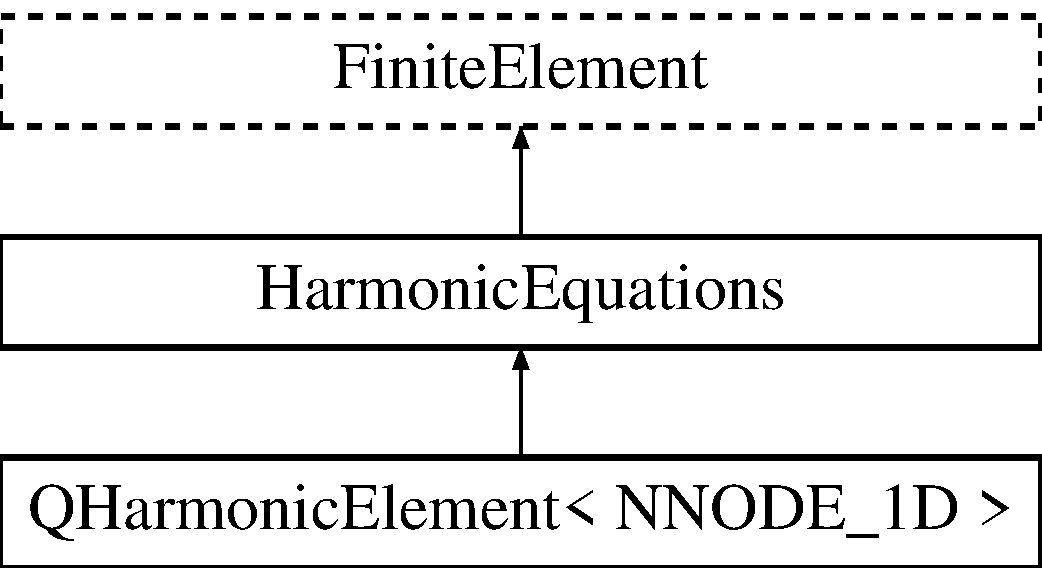
\includegraphics[height=3.000000cm]{classHarmonicEquations}
\end{center}
\end{figure}
\subsection*{Public Member Functions}
\begin{DoxyCompactItemize}
\item 
\hyperlink{classHarmonicEquations_a288d1c0777b2cf5360e1310d48f8c217}{Harmonic\+Equations} ()
\begin{DoxyCompactList}\small\item\em Empty Constructor. \end{DoxyCompactList}\item 
virtual double \hyperlink{classHarmonicEquations_ab801694318460d371e066419263995d7}{u} (const unsigned \&n) const
\begin{DoxyCompactList}\small\item\em Access function\+: Eigenfunction value at local node n Note that solving the eigenproblem does not assign values to this storage space. It is used for output purposes only. \end{DoxyCompactList}\item 
void \hyperlink{classHarmonicEquations_abe34292042ce1394f8979618ee10f354}{output} (ostream \&outfile)
\begin{DoxyCompactList}\small\item\em Output the eigenfunction with default number of plot points. \end{DoxyCompactList}\item 
void \hyperlink{classHarmonicEquations_ab5e53f73bbefb6509ad014c3b236e31f}{output} (ostream \&outfile, const unsigned \&nplot)
\begin{DoxyCompactList}\small\item\em Output FE representation of soln\+: x,y,u or x,y,z,u at Nplot plot points. \end{DoxyCompactList}\item 
void \hyperlink{classHarmonicEquations_a0b756d9ac8dd9c7b9b7785c06f4fce77}{fill\+\_\+in\+\_\+contribution\+\_\+to\+\_\+jacobian\+\_\+and\+\_\+mass\+\_\+matrix} (Vector$<$ double $>$ \&residuals, Dense\+Matrix$<$ double $>$ \&jacobian, Dense\+Matrix$<$ double $>$ \&mass\+\_\+matrix)
\begin{DoxyCompactList}\small\item\em Assemble the contributions to the jacobian and mass matrices. \end{DoxyCompactList}\item 
double \hyperlink{classHarmonicEquations_a5d1ba796d0b62885cab6ef47a83f6b08}{interpolated\+\_\+u} (const Vector$<$ double $>$ \&s) const
\begin{DoxyCompactList}\small\item\em Return FE representation of function value u(s) at local coordinate s. \end{DoxyCompactList}\end{DoxyCompactItemize}
\subsection*{Protected Member Functions}
\begin{DoxyCompactItemize}
\item 
virtual double \hyperlink{classHarmonicEquations_ae013637e60841f46cf4c452ee3469163}{dshape\+\_\+eulerian} (const Vector$<$ double $>$ \&s, Shape \&psi, D\+Shape \&dpsidx) const =0
\begin{DoxyCompactList}\small\item\em Shape/test functions and derivs w.\+r.\+t. to global coords at local coord. s; return Jacobian of mapping. \end{DoxyCompactList}\item 
virtual double \hyperlink{classHarmonicEquations_aaf04ba09dd948dcb0efb8e7e43da9736}{dshape\+\_\+eulerian\+\_\+at\+\_\+knot} (const unsigned \&ipt, Shape \&psi, D\+Shape \&dpsidx) const =0
\begin{DoxyCompactList}\small\item\em Shape/test functions and derivs w.\+r.\+t. to global coords at integration point ipt; return Jacobian of mapping. \end{DoxyCompactList}\item 
virtual int \hyperlink{classHarmonicEquations_a89ff4c11fade61386745931722a75e1d}{u\+\_\+local\+\_\+eqn} (const unsigned \&n)
\begin{DoxyCompactList}\small\item\em Access function that returns the local equation number of the unknown in the problem. Default is to assume that it is the first (only) value stored at the node. \end{DoxyCompactList}\end{DoxyCompactItemize}


\subsection{Detailed Description}
A class for all elements that solve the simple one-\/dimensional eigenvalue problem \[ \frac{\partial^2 u}{\partial x_i^2} + \lambda u = 0 \] These elements are very closely related to the Poisson elements and could inherit from them. They are here developed from scratch for pedagogical purposes. This class contains the generic maths. Shape functions, geometric mapping etc. must get implemented in derived class. 

Definition at line 74 of file harmonic.\+cc.



\subsection{Constructor \& Destructor Documentation}
\mbox{\Hypertarget{classHarmonicEquations_a288d1c0777b2cf5360e1310d48f8c217}\label{classHarmonicEquations_a288d1c0777b2cf5360e1310d48f8c217}} 
\index{Harmonic\+Equations@{Harmonic\+Equations}!Harmonic\+Equations@{Harmonic\+Equations}}
\index{Harmonic\+Equations@{Harmonic\+Equations}!Harmonic\+Equations@{Harmonic\+Equations}}
\subsubsection{\texorpdfstring{Harmonic\+Equations()}{HarmonicEquations()}}
{\footnotesize\ttfamily Harmonic\+Equations\+::\+Harmonic\+Equations (\begin{DoxyParamCaption}{ }\end{DoxyParamCaption})\hspace{0.3cm}{\ttfamily [inline]}}



Empty Constructor. 



Definition at line 79 of file harmonic.\+cc.



\subsection{Member Function Documentation}
\mbox{\Hypertarget{classHarmonicEquations_ae013637e60841f46cf4c452ee3469163}\label{classHarmonicEquations_ae013637e60841f46cf4c452ee3469163}} 
\index{Harmonic\+Equations@{Harmonic\+Equations}!dshape\+\_\+eulerian@{dshape\+\_\+eulerian}}
\index{dshape\+\_\+eulerian@{dshape\+\_\+eulerian}!Harmonic\+Equations@{Harmonic\+Equations}}
\subsubsection{\texorpdfstring{dshape\+\_\+eulerian()}{dshape\_eulerian()}}
{\footnotesize\ttfamily virtual double Harmonic\+Equations\+::dshape\+\_\+eulerian (\begin{DoxyParamCaption}\item[{const Vector$<$ double $>$ \&}]{s,  }\item[{Shape \&}]{psi,  }\item[{D\+Shape \&}]{dpsidx }\end{DoxyParamCaption}) const\hspace{0.3cm}{\ttfamily [protected]}, {\ttfamily [pure virtual]}}



Shape/test functions and derivs w.\+r.\+t. to global coords at local coord. s; return Jacobian of mapping. 



Implemented in \hyperlink{classQHarmonicElement_a206b7334e82cb563d7d575deb9f755b1}{Q\+Harmonic\+Element$<$ N\+N\+O\+D\+E\+\_\+1\+D $>$}.

\mbox{\Hypertarget{classHarmonicEquations_aaf04ba09dd948dcb0efb8e7e43da9736}\label{classHarmonicEquations_aaf04ba09dd948dcb0efb8e7e43da9736}} 
\index{Harmonic\+Equations@{Harmonic\+Equations}!dshape\+\_\+eulerian\+\_\+at\+\_\+knot@{dshape\+\_\+eulerian\+\_\+at\+\_\+knot}}
\index{dshape\+\_\+eulerian\+\_\+at\+\_\+knot@{dshape\+\_\+eulerian\+\_\+at\+\_\+knot}!Harmonic\+Equations@{Harmonic\+Equations}}
\subsubsection{\texorpdfstring{dshape\+\_\+eulerian\+\_\+at\+\_\+knot()}{dshape\_eulerian\_at\_knot()}}
{\footnotesize\ttfamily virtual double Harmonic\+Equations\+::dshape\+\_\+eulerian\+\_\+at\+\_\+knot (\begin{DoxyParamCaption}\item[{const unsigned \&}]{ipt,  }\item[{Shape \&}]{psi,  }\item[{D\+Shape \&}]{dpsidx }\end{DoxyParamCaption}) const\hspace{0.3cm}{\ttfamily [protected]}, {\ttfamily [pure virtual]}}



Shape/test functions and derivs w.\+r.\+t. to global coords at integration point ipt; return Jacobian of mapping. 



Implemented in \hyperlink{classQHarmonicElement_a6b11b5a42bd20c4e1d1e9840ba22a80a}{Q\+Harmonic\+Element$<$ N\+N\+O\+D\+E\+\_\+1\+D $>$}.

\mbox{\Hypertarget{classHarmonicEquations_a0b756d9ac8dd9c7b9b7785c06f4fce77}\label{classHarmonicEquations_a0b756d9ac8dd9c7b9b7785c06f4fce77}} 
\index{Harmonic\+Equations@{Harmonic\+Equations}!fill\+\_\+in\+\_\+contribution\+\_\+to\+\_\+jacobian\+\_\+and\+\_\+mass\+\_\+matrix@{fill\+\_\+in\+\_\+contribution\+\_\+to\+\_\+jacobian\+\_\+and\+\_\+mass\+\_\+matrix}}
\index{fill\+\_\+in\+\_\+contribution\+\_\+to\+\_\+jacobian\+\_\+and\+\_\+mass\+\_\+matrix@{fill\+\_\+in\+\_\+contribution\+\_\+to\+\_\+jacobian\+\_\+and\+\_\+mass\+\_\+matrix}!Harmonic\+Equations@{Harmonic\+Equations}}
\subsubsection{\texorpdfstring{fill\+\_\+in\+\_\+contribution\+\_\+to\+\_\+jacobian\+\_\+and\+\_\+mass\+\_\+matrix()}{fill\_in\_contribution\_to\_jacobian\_and\_mass\_matrix()}}
{\footnotesize\ttfamily void Harmonic\+Equations\+::fill\+\_\+in\+\_\+contribution\+\_\+to\+\_\+jacobian\+\_\+and\+\_\+mass\+\_\+matrix (\begin{DoxyParamCaption}\item[{Vector$<$ double $>$ \&}]{residuals,  }\item[{Dense\+Matrix$<$ double $>$ \&}]{jacobian,  }\item[{Dense\+Matrix$<$ double $>$ \&}]{mass\+\_\+matrix }\end{DoxyParamCaption})\hspace{0.3cm}{\ttfamily [inline]}}



Assemble the contributions to the jacobian and mass matrices. 



Definition at line 119 of file harmonic.\+cc.

\mbox{\Hypertarget{classHarmonicEquations_a5d1ba796d0b62885cab6ef47a83f6b08}\label{classHarmonicEquations_a5d1ba796d0b62885cab6ef47a83f6b08}} 
\index{Harmonic\+Equations@{Harmonic\+Equations}!interpolated\+\_\+u@{interpolated\+\_\+u}}
\index{interpolated\+\_\+u@{interpolated\+\_\+u}!Harmonic\+Equations@{Harmonic\+Equations}}
\subsubsection{\texorpdfstring{interpolated\+\_\+u()}{interpolated\_u()}}
{\footnotesize\ttfamily double Harmonic\+Equations\+::interpolated\+\_\+u (\begin{DoxyParamCaption}\item[{const Vector$<$ double $>$ \&}]{s }\end{DoxyParamCaption}) const\hspace{0.3cm}{\ttfamily [inline]}}



Return FE representation of function value u(s) at local coordinate s. 



Definition at line 174 of file harmonic.\+cc.

\mbox{\Hypertarget{classHarmonicEquations_abe34292042ce1394f8979618ee10f354}\label{classHarmonicEquations_abe34292042ce1394f8979618ee10f354}} 
\index{Harmonic\+Equations@{Harmonic\+Equations}!output@{output}}
\index{output@{output}!Harmonic\+Equations@{Harmonic\+Equations}}
\subsubsection{\texorpdfstring{output()}{output()}\hspace{0.1cm}{\footnotesize\ttfamily [1/2]}}
{\footnotesize\ttfamily void Harmonic\+Equations\+::output (\begin{DoxyParamCaption}\item[{ostream \&}]{outfile }\end{DoxyParamCaption})\hspace{0.3cm}{\ttfamily [inline]}}



Output the eigenfunction with default number of plot points. 



Definition at line 88 of file harmonic.\+cc.



Referenced by Q\+Harmonic\+Element$<$ N\+N\+O\+D\+E\+\_\+1\+D $>$\+::output().

\mbox{\Hypertarget{classHarmonicEquations_ab5e53f73bbefb6509ad014c3b236e31f}\label{classHarmonicEquations_ab5e53f73bbefb6509ad014c3b236e31f}} 
\index{Harmonic\+Equations@{Harmonic\+Equations}!output@{output}}
\index{output@{output}!Harmonic\+Equations@{Harmonic\+Equations}}
\subsubsection{\texorpdfstring{output()}{output()}\hspace{0.1cm}{\footnotesize\ttfamily [2/2]}}
{\footnotesize\ttfamily void Harmonic\+Equations\+::output (\begin{DoxyParamCaption}\item[{ostream \&}]{outfile,  }\item[{const unsigned \&}]{nplot }\end{DoxyParamCaption})\hspace{0.3cm}{\ttfamily [inline]}}



Output FE representation of soln\+: x,y,u or x,y,z,u at Nplot plot points. 



Definition at line 96 of file harmonic.\+cc.

\mbox{\Hypertarget{classHarmonicEquations_ab801694318460d371e066419263995d7}\label{classHarmonicEquations_ab801694318460d371e066419263995d7}} 
\index{Harmonic\+Equations@{Harmonic\+Equations}!u@{u}}
\index{u@{u}!Harmonic\+Equations@{Harmonic\+Equations}}
\subsubsection{\texorpdfstring{u()}{u()}}
{\footnotesize\ttfamily virtual double Harmonic\+Equations\+::u (\begin{DoxyParamCaption}\item[{const unsigned \&}]{n }\end{DoxyParamCaption}) const\hspace{0.3cm}{\ttfamily [inline]}, {\ttfamily [virtual]}}



Access function\+: Eigenfunction value at local node n Note that solving the eigenproblem does not assign values to this storage space. It is used for output purposes only. 



Definition at line 84 of file harmonic.\+cc.

\mbox{\Hypertarget{classHarmonicEquations_a89ff4c11fade61386745931722a75e1d}\label{classHarmonicEquations_a89ff4c11fade61386745931722a75e1d}} 
\index{Harmonic\+Equations@{Harmonic\+Equations}!u\+\_\+local\+\_\+eqn@{u\+\_\+local\+\_\+eqn}}
\index{u\+\_\+local\+\_\+eqn@{u\+\_\+local\+\_\+eqn}!Harmonic\+Equations@{Harmonic\+Equations}}
\subsubsection{\texorpdfstring{u\+\_\+local\+\_\+eqn()}{u\_local\_eqn()}}
{\footnotesize\ttfamily virtual int Harmonic\+Equations\+::u\+\_\+local\+\_\+eqn (\begin{DoxyParamCaption}\item[{const unsigned \&}]{n }\end{DoxyParamCaption})\hspace{0.3cm}{\ttfamily [inline]}, {\ttfamily [protected]}, {\ttfamily [virtual]}}



Access function that returns the local equation number of the unknown in the problem. Default is to assume that it is the first (only) value stored at the node. 



Definition at line 211 of file harmonic.\+cc.



The documentation for this class was generated from the following file\+:\begin{DoxyCompactItemize}
\item 
\hyperlink{harmonic_8cc}{harmonic.\+cc}\end{DoxyCompactItemize}

\hypertarget{classHarmonicProblem}{}\section{Harmonic\+Problem$<$ E\+L\+E\+M\+E\+NT, E\+I\+G\+E\+N\+\_\+\+S\+O\+L\+V\+ER $>$ Class Template Reference}
\label{classHarmonicProblem}\index{Harmonic\+Problem$<$ E\+L\+E\+M\+E\+N\+T, E\+I\+G\+E\+N\+\_\+\+S\+O\+L\+V\+E\+R $>$@{Harmonic\+Problem$<$ E\+L\+E\+M\+E\+N\+T, E\+I\+G\+E\+N\+\_\+\+S\+O\+L\+V\+E\+R $>$}}


1D Harmonic problem in unit interval.  


Inheritance diagram for Harmonic\+Problem$<$ E\+L\+E\+M\+E\+NT, E\+I\+G\+E\+N\+\_\+\+S\+O\+L\+V\+ER $>$\+:\begin{figure}[H]
\begin{center}
\leavevmode
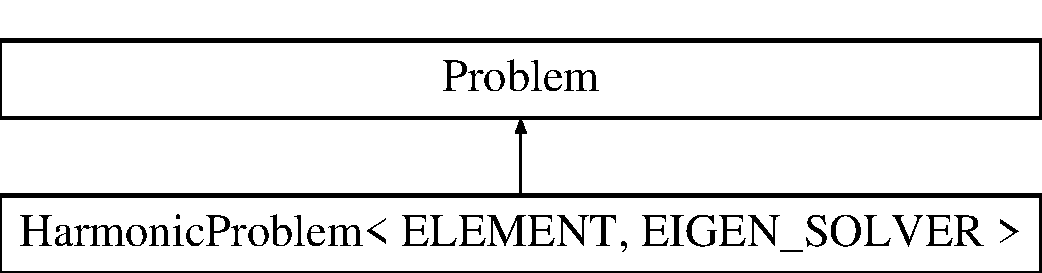
\includegraphics[height=2.000000cm]{classHarmonicProblem}
\end{center}
\end{figure}
\subsection*{Public Member Functions}
\begin{DoxyCompactItemize}
\item 
\hyperlink{classHarmonicProblem_a77a25847f00ae50c83218530149e3e57}{Harmonic\+Problem} (const unsigned \&n\+\_\+element)
\begin{DoxyCompactList}\small\item\em Constructor\+: Pass number of elements and pointer to source function. \end{DoxyCompactList}\item 
\hyperlink{classHarmonicProblem_a929be27d0bb040eef28336b2145b5a59}{$\sim$\+Harmonic\+Problem} ()
\begin{DoxyCompactList}\small\item\em Destructor (empty) \end{DoxyCompactList}\item 
void \hyperlink{classHarmonicProblem_aba2b3fd58a67f03ca0481e426d385c5d}{solve} (const unsigned \&label)
\begin{DoxyCompactList}\small\item\em Solve the problem. \end{DoxyCompactList}\item 
void \hyperlink{classHarmonicProblem_a95e94f87cf4f63e332c09bd9f1bbae7c}{doc\+\_\+solution} (const unsigned \&label)
\begin{DoxyCompactList}\small\item\em Doc the solution, pass the number of the case considered, so that output files can be distinguished. \end{DoxyCompactList}\end{DoxyCompactItemize}


\subsection{Detailed Description}
\subsubsection*{template$<$class E\+L\+E\+M\+E\+NT, class E\+I\+G\+E\+N\+\_\+\+S\+O\+L\+V\+ER$>$\newline
class Harmonic\+Problem$<$ E\+L\+E\+M\+E\+N\+T, E\+I\+G\+E\+N\+\_\+\+S\+O\+L\+V\+E\+R $>$}

1D Harmonic problem in unit interval. 

Definition at line 272 of file harmonic.\+cc.



\subsection{Constructor \& Destructor Documentation}
\mbox{\Hypertarget{classHarmonicProblem_a77a25847f00ae50c83218530149e3e57}\label{classHarmonicProblem_a77a25847f00ae50c83218530149e3e57}} 
\index{Harmonic\+Problem@{Harmonic\+Problem}!Harmonic\+Problem@{Harmonic\+Problem}}
\index{Harmonic\+Problem@{Harmonic\+Problem}!Harmonic\+Problem@{Harmonic\+Problem}}
\subsubsection{\texorpdfstring{Harmonic\+Problem()}{HarmonicProblem()}}
{\footnotesize\ttfamily template$<$class E\+L\+E\+M\+E\+NT , class E\+I\+G\+E\+N\+\_\+\+S\+O\+L\+V\+ER $>$ \\
\hyperlink{classHarmonicProblem}{Harmonic\+Problem}$<$ E\+L\+E\+M\+E\+NT, E\+I\+G\+E\+N\+\_\+\+S\+O\+L\+V\+ER $>$\+::\hyperlink{classHarmonicProblem}{Harmonic\+Problem} (\begin{DoxyParamCaption}\item[{const unsigned \&}]{n\+\_\+element }\end{DoxyParamCaption})}



Constructor\+: Pass number of elements and pointer to source function. 

Constructor for 1D Harmonic problem in unit interval. Discretise the 1D domain with n\+\_\+element elements of type E\+L\+E\+M\+E\+NT. Specify function pointer to source function. 

Definition at line 299 of file harmonic.\+cc.

\mbox{\Hypertarget{classHarmonicProblem_a929be27d0bb040eef28336b2145b5a59}\label{classHarmonicProblem_a929be27d0bb040eef28336b2145b5a59}} 
\index{Harmonic\+Problem@{Harmonic\+Problem}!````~Harmonic\+Problem@{$\sim$\+Harmonic\+Problem}}
\index{````~Harmonic\+Problem@{$\sim$\+Harmonic\+Problem}!Harmonic\+Problem@{Harmonic\+Problem}}
\subsubsection{\texorpdfstring{$\sim$\+Harmonic\+Problem()}{~HarmonicProblem()}}
{\footnotesize\ttfamily template$<$class E\+L\+E\+M\+E\+NT, class E\+I\+G\+E\+N\+\_\+\+S\+O\+L\+V\+ER$>$ \\
\hyperlink{classHarmonicProblem}{Harmonic\+Problem}$<$ E\+L\+E\+M\+E\+NT, E\+I\+G\+E\+N\+\_\+\+S\+O\+L\+V\+ER $>$\+::$\sim$\hyperlink{classHarmonicProblem}{Harmonic\+Problem} (\begin{DoxyParamCaption}{ }\end{DoxyParamCaption})\hspace{0.3cm}{\ttfamily [inline]}}



Destructor (empty) 



Definition at line 280 of file harmonic.\+cc.



\subsection{Member Function Documentation}
\mbox{\Hypertarget{classHarmonicProblem_a95e94f87cf4f63e332c09bd9f1bbae7c}\label{classHarmonicProblem_a95e94f87cf4f63e332c09bd9f1bbae7c}} 
\index{Harmonic\+Problem@{Harmonic\+Problem}!doc\+\_\+solution@{doc\+\_\+solution}}
\index{doc\+\_\+solution@{doc\+\_\+solution}!Harmonic\+Problem@{Harmonic\+Problem}}
\subsubsection{\texorpdfstring{doc\+\_\+solution()}{doc\_solution()}}
{\footnotesize\ttfamily template$<$class E\+L\+E\+M\+E\+NT , class E\+I\+G\+E\+N\+\_\+\+S\+O\+L\+V\+ER $>$ \\
void \hyperlink{classHarmonicProblem}{Harmonic\+Problem}$<$ E\+L\+E\+M\+E\+NT, E\+I\+G\+E\+N\+\_\+\+S\+O\+L\+V\+ER $>$\+::doc\+\_\+solution (\begin{DoxyParamCaption}\item[{const unsigned \&}]{label }\end{DoxyParamCaption})}



Doc the solution, pass the number of the case considered, so that output files can be distinguished. 

Doc the solution in tecplot format. Label files with label. 

Definition at line 338 of file harmonic.\+cc.



References Harmonic\+Problem$<$ E\+L\+E\+M\+E\+N\+T, E\+I\+G\+E\+N\+\_\+\+S\+O\+L\+V\+E\+R $>$\+::solve().

\mbox{\Hypertarget{classHarmonicProblem_aba2b3fd58a67f03ca0481e426d385c5d}\label{classHarmonicProblem_aba2b3fd58a67f03ca0481e426d385c5d}} 
\index{Harmonic\+Problem@{Harmonic\+Problem}!solve@{solve}}
\index{solve@{solve}!Harmonic\+Problem@{Harmonic\+Problem}}
\subsubsection{\texorpdfstring{solve()}{solve()}}
{\footnotesize\ttfamily template$<$class E\+L\+E\+M\+E\+NT , class E\+I\+G\+E\+N\+\_\+\+S\+O\+L\+V\+ER $>$ \\
void \hyperlink{classHarmonicProblem}{Harmonic\+Problem}$<$ E\+L\+E\+M\+E\+NT, E\+I\+G\+E\+N\+\_\+\+S\+O\+L\+V\+ER $>$\+::solve (\begin{DoxyParamCaption}\item[{const unsigned \&}]{label }\end{DoxyParamCaption})}



Solve the problem. 

Solve the eigenproblem. 

Definition at line 361 of file harmonic.\+cc.



Referenced by Harmonic\+Problem$<$ E\+L\+E\+M\+E\+N\+T, E\+I\+G\+E\+N\+\_\+\+S\+O\+L\+V\+E\+R $>$\+::doc\+\_\+solution(), and main().



The documentation for this class was generated from the following file\+:\begin{DoxyCompactItemize}
\item 
\hyperlink{harmonic_8cc}{harmonic.\+cc}\end{DoxyCompactItemize}

\hypertarget{classQComplexHarmonicElement}{}\section{Q\+Complex\+Harmonic\+Element$<$ N\+N\+O\+D\+E\+\_\+1D $>$ Class Template Reference}
\label{classQComplexHarmonicElement}\index{Q\+Complex\+Harmonic\+Element$<$ N\+N\+O\+D\+E\+\_\+1\+D $>$@{Q\+Complex\+Harmonic\+Element$<$ N\+N\+O\+D\+E\+\_\+1\+D $>$}}
Inheritance diagram for Q\+Complex\+Harmonic\+Element$<$ N\+N\+O\+D\+E\+\_\+1D $>$\+:\begin{figure}[H]
\begin{center}
\leavevmode
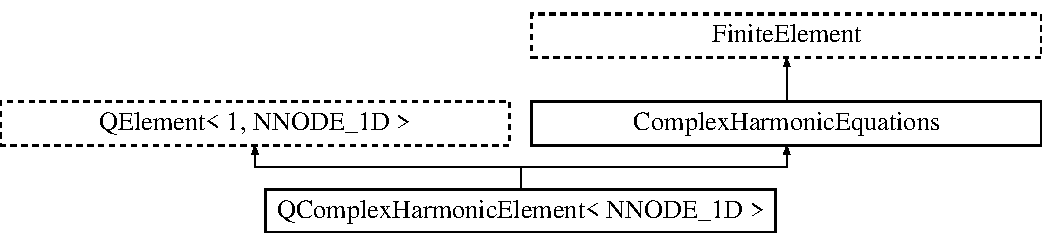
\includegraphics[height=3.000000cm]{classQComplexHarmonicElement}
\end{center}
\end{figure}
\subsection*{Public Member Functions}
\begin{DoxyCompactItemize}
\item 
\hyperlink{classQComplexHarmonicElement_a9f1e88c4b5c7031d77c6f6dd3758de2a}{Q\+Complex\+Harmonic\+Element} ()
\begin{DoxyCompactList}\small\item\em Constructor\+: Call constructors for Q\+Element and Poisson equations. \end{DoxyCompactList}\item 
unsigned \hyperlink{classQComplexHarmonicElement_a3f1d68324e9d8b9e143044d716c72a87}{required\+\_\+nvalue} (const unsigned \&n) const
\begin{DoxyCompactList}\small\item\em Required \# of `values\textquotesingle{} (pinned or dofs) at node n. Here there are two (u and w) \end{DoxyCompactList}\item 
void \hyperlink{classQComplexHarmonicElement_a8c45d7281a7bc7e2e2d53a7f87339ca4}{output} (ostream \&outfile)
\begin{DoxyCompactList}\small\item\em Output function overloaded from \hyperlink{classComplexHarmonicEquations}{Complex\+Harmonic\+Equations}. \end{DoxyCompactList}\item 
void \hyperlink{classQComplexHarmonicElement_a7f63f8532a6295a3ba86f94355f889b8}{output} (ostream \&outfile, const unsigned \&Nplot)
\begin{DoxyCompactList}\small\item\em Output function overloaded from \hyperlink{classComplexHarmonicEquations}{Complex\+Harmonic\+Equations}. \end{DoxyCompactList}\end{DoxyCompactItemize}
\subsection*{Protected Member Functions}
\begin{DoxyCompactItemize}
\item 
double \hyperlink{classQComplexHarmonicElement_a7c97d4e8c5433a44640d30c936d69ffb}{dshape\+\_\+eulerian} (const Vector$<$ double $>$ \&s, Shape \&psi, D\+Shape \&dpsidx) const
\begin{DoxyCompactList}\small\item\em Shape, test functions \& derivs. w.\+r.\+t. to global coords. Return Jacobian. \end{DoxyCompactList}\item 
double \hyperlink{classQComplexHarmonicElement_a3f8d1d9396135d4d86f416dcf6c23904}{dshape\+\_\+eulerian\+\_\+at\+\_\+knot} (const unsigned \&ipt, Shape \&psi, D\+Shape \&dpsidx) const
\begin{DoxyCompactList}\small\item\em Shape, test functions \& derivs. w.\+r.\+t. to global coords. at integration point ipt. Return Jacobian. \end{DoxyCompactList}\end{DoxyCompactItemize}


\subsection{Detailed Description}
\subsubsection*{template$<$unsigned N\+N\+O\+D\+E\+\_\+1D$>$\newline
class Q\+Complex\+Harmonic\+Element$<$ N\+N\+O\+D\+E\+\_\+1\+D $>$}

Q\+Complex\+Harmonic\+Element$<$\+N\+N\+O\+D\+E\+\_\+1\+D$>$ elements are 1D Elements with N\+N\+O\+D\+E\+\_\+1D nodal points that are used to solve the Complex\+Harmonic eigenvalue Problem described by \hyperlink{classComplexHarmonicEquations}{Complex\+Harmonic\+Equations}. 

Definition at line 306 of file complex\+\_\+harmonic.\+cc.



\subsection{Constructor \& Destructor Documentation}
\mbox{\Hypertarget{classQComplexHarmonicElement_a9f1e88c4b5c7031d77c6f6dd3758de2a}\label{classQComplexHarmonicElement_a9f1e88c4b5c7031d77c6f6dd3758de2a}} 
\index{Q\+Complex\+Harmonic\+Element@{Q\+Complex\+Harmonic\+Element}!Q\+Complex\+Harmonic\+Element@{Q\+Complex\+Harmonic\+Element}}
\index{Q\+Complex\+Harmonic\+Element@{Q\+Complex\+Harmonic\+Element}!Q\+Complex\+Harmonic\+Element@{Q\+Complex\+Harmonic\+Element}}
\subsubsection{\texorpdfstring{Q\+Complex\+Harmonic\+Element()}{QComplexHarmonicElement()}}
{\footnotesize\ttfamily template$<$unsigned N\+N\+O\+D\+E\+\_\+1D$>$ \\
\hyperlink{classQComplexHarmonicElement}{Q\+Complex\+Harmonic\+Element}$<$ N\+N\+O\+D\+E\+\_\+1D $>$\+::\hyperlink{classQComplexHarmonicElement}{Q\+Complex\+Harmonic\+Element} (\begin{DoxyParamCaption}{ }\end{DoxyParamCaption})\hspace{0.3cm}{\ttfamily [inline]}}



Constructor\+: Call constructors for Q\+Element and Poisson equations. 



Definition at line 314 of file complex\+\_\+harmonic.\+cc.



\subsection{Member Function Documentation}
\mbox{\Hypertarget{classQComplexHarmonicElement_a7c97d4e8c5433a44640d30c936d69ffb}\label{classQComplexHarmonicElement_a7c97d4e8c5433a44640d30c936d69ffb}} 
\index{Q\+Complex\+Harmonic\+Element@{Q\+Complex\+Harmonic\+Element}!dshape\+\_\+eulerian@{dshape\+\_\+eulerian}}
\index{dshape\+\_\+eulerian@{dshape\+\_\+eulerian}!Q\+Complex\+Harmonic\+Element@{Q\+Complex\+Harmonic\+Element}}
\subsubsection{\texorpdfstring{dshape\+\_\+eulerian()}{dshape\_eulerian()}}
{\footnotesize\ttfamily template$<$unsigned N\+N\+O\+D\+E\+\_\+1D$>$ \\
double \hyperlink{classQComplexHarmonicElement}{Q\+Complex\+Harmonic\+Element}$<$ N\+N\+O\+D\+E\+\_\+1D $>$\+::dshape\+\_\+eulerian (\begin{DoxyParamCaption}\item[{const Vector$<$ double $>$ \&}]{s,  }\item[{Shape \&}]{psi,  }\item[{D\+Shape \&}]{dpsidx }\end{DoxyParamCaption}) const\hspace{0.3cm}{\ttfamily [inline]}, {\ttfamily [protected]}, {\ttfamily [virtual]}}



Shape, test functions \& derivs. w.\+r.\+t. to global coords. Return Jacobian. 



Implements \hyperlink{classComplexHarmonicEquations_a59048c598e2fba3e11aa5985ffaf4d76}{Complex\+Harmonic\+Equations}.



Definition at line 333 of file complex\+\_\+harmonic.\+cc.

\mbox{\Hypertarget{classQComplexHarmonicElement_a3f8d1d9396135d4d86f416dcf6c23904}\label{classQComplexHarmonicElement_a3f8d1d9396135d4d86f416dcf6c23904}} 
\index{Q\+Complex\+Harmonic\+Element@{Q\+Complex\+Harmonic\+Element}!dshape\+\_\+eulerian\+\_\+at\+\_\+knot@{dshape\+\_\+eulerian\+\_\+at\+\_\+knot}}
\index{dshape\+\_\+eulerian\+\_\+at\+\_\+knot@{dshape\+\_\+eulerian\+\_\+at\+\_\+knot}!Q\+Complex\+Harmonic\+Element@{Q\+Complex\+Harmonic\+Element}}
\subsubsection{\texorpdfstring{dshape\+\_\+eulerian\+\_\+at\+\_\+knot()}{dshape\_eulerian\_at\_knot()}}
{\footnotesize\ttfamily template$<$unsigned N\+N\+O\+D\+E\+\_\+1D$>$ \\
double \hyperlink{classQComplexHarmonicElement}{Q\+Complex\+Harmonic\+Element}$<$ N\+N\+O\+D\+E\+\_\+1D $>$\+::dshape\+\_\+eulerian\+\_\+at\+\_\+knot (\begin{DoxyParamCaption}\item[{const unsigned \&}]{ipt,  }\item[{Shape \&}]{psi,  }\item[{D\+Shape \&}]{dpsidx }\end{DoxyParamCaption}) const\hspace{0.3cm}{\ttfamily [inline]}, {\ttfamily [protected]}, {\ttfamily [virtual]}}



Shape, test functions \& derivs. w.\+r.\+t. to global coords. at integration point ipt. Return Jacobian. 



Implements \hyperlink{classComplexHarmonicEquations_a60c71828f2d4c1c2363dcb1d1f334fff}{Complex\+Harmonic\+Equations}.



Definition at line 341 of file complex\+\_\+harmonic.\+cc.

\mbox{\Hypertarget{classQComplexHarmonicElement_a8c45d7281a7bc7e2e2d53a7f87339ca4}\label{classQComplexHarmonicElement_a8c45d7281a7bc7e2e2d53a7f87339ca4}} 
\index{Q\+Complex\+Harmonic\+Element@{Q\+Complex\+Harmonic\+Element}!output@{output}}
\index{output@{output}!Q\+Complex\+Harmonic\+Element@{Q\+Complex\+Harmonic\+Element}}
\subsubsection{\texorpdfstring{output()}{output()}\hspace{0.1cm}{\footnotesize\ttfamily [1/2]}}
{\footnotesize\ttfamily template$<$unsigned N\+N\+O\+D\+E\+\_\+1D$>$ \\
void \hyperlink{classQComplexHarmonicElement}{Q\+Complex\+Harmonic\+Element}$<$ N\+N\+O\+D\+E\+\_\+1D $>$\+::output (\begin{DoxyParamCaption}\item[{ostream \&}]{outfile }\end{DoxyParamCaption})\hspace{0.3cm}{\ttfamily [inline]}}



Output function overloaded from \hyperlink{classComplexHarmonicEquations}{Complex\+Harmonic\+Equations}. 



Definition at line 322 of file complex\+\_\+harmonic.\+cc.



References Complex\+Harmonic\+Equations\+::output().

\mbox{\Hypertarget{classQComplexHarmonicElement_a7f63f8532a6295a3ba86f94355f889b8}\label{classQComplexHarmonicElement_a7f63f8532a6295a3ba86f94355f889b8}} 
\index{Q\+Complex\+Harmonic\+Element@{Q\+Complex\+Harmonic\+Element}!output@{output}}
\index{output@{output}!Q\+Complex\+Harmonic\+Element@{Q\+Complex\+Harmonic\+Element}}
\subsubsection{\texorpdfstring{output()}{output()}\hspace{0.1cm}{\footnotesize\ttfamily [2/2]}}
{\footnotesize\ttfamily template$<$unsigned N\+N\+O\+D\+E\+\_\+1D$>$ \\
void \hyperlink{classQComplexHarmonicElement}{Q\+Complex\+Harmonic\+Element}$<$ N\+N\+O\+D\+E\+\_\+1D $>$\+::output (\begin{DoxyParamCaption}\item[{ostream \&}]{outfile,  }\item[{const unsigned \&}]{Nplot }\end{DoxyParamCaption})\hspace{0.3cm}{\ttfamily [inline]}}



Output function overloaded from \hyperlink{classComplexHarmonicEquations}{Complex\+Harmonic\+Equations}. 



Definition at line 326 of file complex\+\_\+harmonic.\+cc.



References Complex\+Harmonic\+Equations\+::output().

\mbox{\Hypertarget{classQComplexHarmonicElement_a3f1d68324e9d8b9e143044d716c72a87}\label{classQComplexHarmonicElement_a3f1d68324e9d8b9e143044d716c72a87}} 
\index{Q\+Complex\+Harmonic\+Element@{Q\+Complex\+Harmonic\+Element}!required\+\_\+nvalue@{required\+\_\+nvalue}}
\index{required\+\_\+nvalue@{required\+\_\+nvalue}!Q\+Complex\+Harmonic\+Element@{Q\+Complex\+Harmonic\+Element}}
\subsubsection{\texorpdfstring{required\+\_\+nvalue()}{required\_nvalue()}}
{\footnotesize\ttfamily template$<$unsigned N\+N\+O\+D\+E\+\_\+1D$>$ \\
unsigned \hyperlink{classQComplexHarmonicElement}{Q\+Complex\+Harmonic\+Element}$<$ N\+N\+O\+D\+E\+\_\+1D $>$\+::required\+\_\+nvalue (\begin{DoxyParamCaption}\item[{const unsigned \&}]{n }\end{DoxyParamCaption}) const\hspace{0.3cm}{\ttfamily [inline]}}



Required \# of `values\textquotesingle{} (pinned or dofs) at node n. Here there are two (u and w) 



Definition at line 319 of file complex\+\_\+harmonic.\+cc.



The documentation for this class was generated from the following file\+:\begin{DoxyCompactItemize}
\item 
\hyperlink{complex__harmonic_8cc}{complex\+\_\+harmonic.\+cc}\end{DoxyCompactItemize}

\hypertarget{classQHarmonicElement}{}\section{Q\+Harmonic\+Element$<$ N\+N\+O\+D\+E\+\_\+1D $>$ Class Template Reference}
\label{classQHarmonicElement}\index{Q\+Harmonic\+Element$<$ N\+N\+O\+D\+E\+\_\+1\+D $>$@{Q\+Harmonic\+Element$<$ N\+N\+O\+D\+E\+\_\+1\+D $>$}}
Inheritance diagram for Q\+Harmonic\+Element$<$ N\+N\+O\+D\+E\+\_\+1D $>$\+:\begin{figure}[H]
\begin{center}
\leavevmode
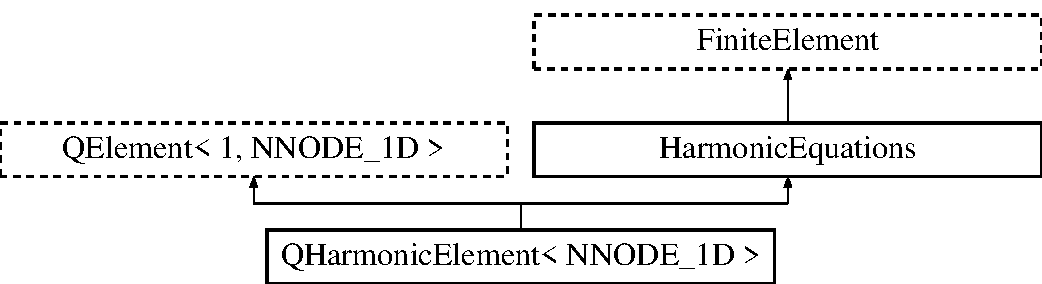
\includegraphics[height=3.000000cm]{classQHarmonicElement}
\end{center}
\end{figure}
\subsection*{Public Member Functions}
\begin{DoxyCompactItemize}
\item 
\hyperlink{classQHarmonicElement_a0e7480a0064b51e87ba197551bb10373}{Q\+Harmonic\+Element} ()
\begin{DoxyCompactList}\small\item\em Constructor\+: Call constructors for Q\+Element and Poisson equations. \end{DoxyCompactList}\item 
unsigned \hyperlink{classQHarmonicElement_a8574a452983b15fb2b4d40ec4ef3e890}{required\+\_\+nvalue} (const unsigned \&n) const
\begin{DoxyCompactList}\small\item\em Required \# of `values\textquotesingle{} (pinned or dofs) at node n. \end{DoxyCompactList}\item 
void \hyperlink{classQHarmonicElement_a8b38012f3d62ef419c359f5e545e5f85}{output} (ostream \&outfile)
\begin{DoxyCompactList}\small\item\em Output function overloaded from \hyperlink{classHarmonicEquations}{Harmonic\+Equations}. \end{DoxyCompactList}\item 
void \hyperlink{classQHarmonicElement_a25cda8268943ebba984da16b07544e89}{output} (ostream \&outfile, const unsigned \&Nplot)
\begin{DoxyCompactList}\small\item\em Output function overloaded from \hyperlink{classHarmonicEquations}{Harmonic\+Equations}. \end{DoxyCompactList}\end{DoxyCompactItemize}
\subsection*{Protected Member Functions}
\begin{DoxyCompactItemize}
\item 
double \hyperlink{classQHarmonicElement_a206b7334e82cb563d7d575deb9f755b1}{dshape\+\_\+eulerian} (const Vector$<$ double $>$ \&s, Shape \&psi, D\+Shape \&dpsidx) const
\begin{DoxyCompactList}\small\item\em Shape, test functions \& derivs. w.\+r.\+t. to global coords. Return Jacobian. \end{DoxyCompactList}\item 
double \hyperlink{classQHarmonicElement_a6b11b5a42bd20c4e1d1e9840ba22a80a}{dshape\+\_\+eulerian\+\_\+at\+\_\+knot} (const unsigned \&ipt, Shape \&psi, D\+Shape \&dpsidx) const
\begin{DoxyCompactList}\small\item\em Shape, test functions \& derivs. w.\+r.\+t. to global coords. at integration point ipt. Return Jacobian. \end{DoxyCompactList}\end{DoxyCompactItemize}


\subsection{Detailed Description}
\subsubsection*{template$<$unsigned N\+N\+O\+D\+E\+\_\+1D$>$\newline
class Q\+Harmonic\+Element$<$ N\+N\+O\+D\+E\+\_\+1\+D $>$}

Q\+Harmonic\+Element$<$\+N\+N\+O\+D\+E\+\_\+1\+D$>$ elements are 1D Elements with N\+N\+O\+D\+E\+\_\+1D nodal points that are used to solve the Harmonic eigenvalue Problem described by \hyperlink{classHarmonicEquations}{Harmonic\+Equations}. 

Definition at line 226 of file harmonic.\+cc.



\subsection{Constructor \& Destructor Documentation}
\mbox{\Hypertarget{classQHarmonicElement_a0e7480a0064b51e87ba197551bb10373}\label{classQHarmonicElement_a0e7480a0064b51e87ba197551bb10373}} 
\index{Q\+Harmonic\+Element@{Q\+Harmonic\+Element}!Q\+Harmonic\+Element@{Q\+Harmonic\+Element}}
\index{Q\+Harmonic\+Element@{Q\+Harmonic\+Element}!Q\+Harmonic\+Element@{Q\+Harmonic\+Element}}
\subsubsection{\texorpdfstring{Q\+Harmonic\+Element()}{QHarmonicElement()}}
{\footnotesize\ttfamily template$<$unsigned N\+N\+O\+D\+E\+\_\+1D$>$ \\
\hyperlink{classQHarmonicElement}{Q\+Harmonic\+Element}$<$ N\+N\+O\+D\+E\+\_\+1D $>$\+::\hyperlink{classQHarmonicElement}{Q\+Harmonic\+Element} (\begin{DoxyParamCaption}{ }\end{DoxyParamCaption})\hspace{0.3cm}{\ttfamily [inline]}}



Constructor\+: Call constructors for Q\+Element and Poisson equations. 



Definition at line 234 of file harmonic.\+cc.



\subsection{Member Function Documentation}
\mbox{\Hypertarget{classQHarmonicElement_a206b7334e82cb563d7d575deb9f755b1}\label{classQHarmonicElement_a206b7334e82cb563d7d575deb9f755b1}} 
\index{Q\+Harmonic\+Element@{Q\+Harmonic\+Element}!dshape\+\_\+eulerian@{dshape\+\_\+eulerian}}
\index{dshape\+\_\+eulerian@{dshape\+\_\+eulerian}!Q\+Harmonic\+Element@{Q\+Harmonic\+Element}}
\subsubsection{\texorpdfstring{dshape\+\_\+eulerian()}{dshape\_eulerian()}}
{\footnotesize\ttfamily template$<$unsigned N\+N\+O\+D\+E\+\_\+1D$>$ \\
double \hyperlink{classQHarmonicElement}{Q\+Harmonic\+Element}$<$ N\+N\+O\+D\+E\+\_\+1D $>$\+::dshape\+\_\+eulerian (\begin{DoxyParamCaption}\item[{const Vector$<$ double $>$ \&}]{s,  }\item[{Shape \&}]{psi,  }\item[{D\+Shape \&}]{dpsidx }\end{DoxyParamCaption}) const\hspace{0.3cm}{\ttfamily [inline]}, {\ttfamily [protected]}, {\ttfamily [virtual]}}



Shape, test functions \& derivs. w.\+r.\+t. to global coords. Return Jacobian. 



Implements \hyperlink{classHarmonicEquations_ae013637e60841f46cf4c452ee3469163}{Harmonic\+Equations}.



Definition at line 252 of file harmonic.\+cc.

\mbox{\Hypertarget{classQHarmonicElement_a6b11b5a42bd20c4e1d1e9840ba22a80a}\label{classQHarmonicElement_a6b11b5a42bd20c4e1d1e9840ba22a80a}} 
\index{Q\+Harmonic\+Element@{Q\+Harmonic\+Element}!dshape\+\_\+eulerian\+\_\+at\+\_\+knot@{dshape\+\_\+eulerian\+\_\+at\+\_\+knot}}
\index{dshape\+\_\+eulerian\+\_\+at\+\_\+knot@{dshape\+\_\+eulerian\+\_\+at\+\_\+knot}!Q\+Harmonic\+Element@{Q\+Harmonic\+Element}}
\subsubsection{\texorpdfstring{dshape\+\_\+eulerian\+\_\+at\+\_\+knot()}{dshape\_eulerian\_at\_knot()}}
{\footnotesize\ttfamily template$<$unsigned N\+N\+O\+D\+E\+\_\+1D$>$ \\
double \hyperlink{classQHarmonicElement}{Q\+Harmonic\+Element}$<$ N\+N\+O\+D\+E\+\_\+1D $>$\+::dshape\+\_\+eulerian\+\_\+at\+\_\+knot (\begin{DoxyParamCaption}\item[{const unsigned \&}]{ipt,  }\item[{Shape \&}]{psi,  }\item[{D\+Shape \&}]{dpsidx }\end{DoxyParamCaption}) const\hspace{0.3cm}{\ttfamily [inline]}, {\ttfamily [protected]}, {\ttfamily [virtual]}}



Shape, test functions \& derivs. w.\+r.\+t. to global coords. at integration point ipt. Return Jacobian. 



Implements \hyperlink{classHarmonicEquations_aaf04ba09dd948dcb0efb8e7e43da9736}{Harmonic\+Equations}.



Definition at line 260 of file harmonic.\+cc.

\mbox{\Hypertarget{classQHarmonicElement_a8b38012f3d62ef419c359f5e545e5f85}\label{classQHarmonicElement_a8b38012f3d62ef419c359f5e545e5f85}} 
\index{Q\+Harmonic\+Element@{Q\+Harmonic\+Element}!output@{output}}
\index{output@{output}!Q\+Harmonic\+Element@{Q\+Harmonic\+Element}}
\subsubsection{\texorpdfstring{output()}{output()}\hspace{0.1cm}{\footnotesize\ttfamily [1/2]}}
{\footnotesize\ttfamily template$<$unsigned N\+N\+O\+D\+E\+\_\+1D$>$ \\
void \hyperlink{classQHarmonicElement}{Q\+Harmonic\+Element}$<$ N\+N\+O\+D\+E\+\_\+1D $>$\+::output (\begin{DoxyParamCaption}\item[{ostream \&}]{outfile }\end{DoxyParamCaption})\hspace{0.3cm}{\ttfamily [inline]}}



Output function overloaded from \hyperlink{classHarmonicEquations}{Harmonic\+Equations}. 



Definition at line 241 of file harmonic.\+cc.



References Harmonic\+Equations\+::output().

\mbox{\Hypertarget{classQHarmonicElement_a25cda8268943ebba984da16b07544e89}\label{classQHarmonicElement_a25cda8268943ebba984da16b07544e89}} 
\index{Q\+Harmonic\+Element@{Q\+Harmonic\+Element}!output@{output}}
\index{output@{output}!Q\+Harmonic\+Element@{Q\+Harmonic\+Element}}
\subsubsection{\texorpdfstring{output()}{output()}\hspace{0.1cm}{\footnotesize\ttfamily [2/2]}}
{\footnotesize\ttfamily template$<$unsigned N\+N\+O\+D\+E\+\_\+1D$>$ \\
void \hyperlink{classQHarmonicElement}{Q\+Harmonic\+Element}$<$ N\+N\+O\+D\+E\+\_\+1D $>$\+::output (\begin{DoxyParamCaption}\item[{ostream \&}]{outfile,  }\item[{const unsigned \&}]{Nplot }\end{DoxyParamCaption})\hspace{0.3cm}{\ttfamily [inline]}}



Output function overloaded from \hyperlink{classHarmonicEquations}{Harmonic\+Equations}. 



Definition at line 245 of file harmonic.\+cc.



References Harmonic\+Equations\+::output().

\mbox{\Hypertarget{classQHarmonicElement_a8574a452983b15fb2b4d40ec4ef3e890}\label{classQHarmonicElement_a8574a452983b15fb2b4d40ec4ef3e890}} 
\index{Q\+Harmonic\+Element@{Q\+Harmonic\+Element}!required\+\_\+nvalue@{required\+\_\+nvalue}}
\index{required\+\_\+nvalue@{required\+\_\+nvalue}!Q\+Harmonic\+Element@{Q\+Harmonic\+Element}}
\subsubsection{\texorpdfstring{required\+\_\+nvalue()}{required\_nvalue()}}
{\footnotesize\ttfamily template$<$unsigned N\+N\+O\+D\+E\+\_\+1D$>$ \\
unsigned \hyperlink{classQHarmonicElement}{Q\+Harmonic\+Element}$<$ N\+N\+O\+D\+E\+\_\+1D $>$\+::required\+\_\+nvalue (\begin{DoxyParamCaption}\item[{const unsigned \&}]{n }\end{DoxyParamCaption}) const\hspace{0.3cm}{\ttfamily [inline]}}



Required \# of `values\textquotesingle{} (pinned or dofs) at node n. 



Definition at line 238 of file harmonic.\+cc.



The documentation for this class was generated from the following file\+:\begin{DoxyCompactItemize}
\item 
\hyperlink{harmonic_8cc}{harmonic.\+cc}\end{DoxyCompactItemize}

\chapter{File Documentation}
\hypertarget{complex__harmonic_8cc}{}\section{complex\+\_\+harmonic.\+cc File Reference}
\label{complex__harmonic_8cc}\index{complex\+\_\+harmonic.\+cc@{complex\+\_\+harmonic.\+cc}}
\subsection*{Classes}
\begin{DoxyCompactItemize}
\item 
class \hyperlink{classComplexLess}{Complex\+Less$<$ T $>$}
\item 
class \hyperlink{classComplexHarmonicEquations}{Complex\+Harmonic\+Equations}
\item 
class \hyperlink{classQComplexHarmonicElement}{Q\+Complex\+Harmonic\+Element$<$ N\+N\+O\+D\+E\+\_\+1\+D $>$}
\item 
class \hyperlink{classComplexHarmonicProblem}{Complex\+Harmonic\+Problem$<$ E\+L\+E\+M\+E\+N\+T, E\+I\+G\+E\+N\+\_\+\+S\+O\+L\+V\+E\+R $>$}
\begin{DoxyCompactList}\small\item\em 1D Complex\+Harmonic problem in unit interval. \end{DoxyCompactList}\end{DoxyCompactItemize}
\subsection*{Namespaces}
\begin{DoxyCompactItemize}
\item 
 \hyperlink{namespaceEigenproblemShift}{Eigenproblem\+Shift}
\begin{DoxyCompactList}\small\item\em Namespace for the shift applied to the eigenproblem. \end{DoxyCompactList}\end{DoxyCompactItemize}
\subsection*{Functions}
\begin{DoxyCompactItemize}
\item 
int \hyperlink{complex__harmonic_8cc_a3c04138a5bfe5d72780bb7e82a18e627}{main} (int argc, char $\ast$$\ast$argv)
\begin{DoxyCompactList}\small\item\em Driver for 1D Poisson problem. \end{DoxyCompactList}\end{DoxyCompactItemize}
\subsection*{Variables}
\begin{DoxyCompactItemize}
\item 
double \hyperlink{namespaceEigenproblemShift_a82e816b5ecba937123c65c5bd953a2fb}{Eigenproblem\+Shift\+::\+Mu} = 6.\+5
\end{DoxyCompactItemize}


\subsection{Function Documentation}
\mbox{\Hypertarget{complex__harmonic_8cc_a3c04138a5bfe5d72780bb7e82a18e627}\label{complex__harmonic_8cc_a3c04138a5bfe5d72780bb7e82a18e627}} 
\index{complex\+\_\+harmonic.\+cc@{complex\+\_\+harmonic.\+cc}!main@{main}}
\index{main@{main}!complex\+\_\+harmonic.\+cc@{complex\+\_\+harmonic.\+cc}}
\subsubsection{\texorpdfstring{main()}{main()}}
{\footnotesize\ttfamily int main (\begin{DoxyParamCaption}\item[{int}]{argc,  }\item[{char $\ast$$\ast$}]{argv }\end{DoxyParamCaption})}



Driver for 1D Poisson problem. 



Definition at line 531 of file complex\+\_\+harmonic.\+cc.



References Complex\+Harmonic\+Problem$<$ E\+L\+E\+M\+E\+N\+T, E\+I\+G\+E\+N\+\_\+\+S\+O\+L\+V\+E\+R $>$\+::solve().


\hypertarget{complex__harmonic_8txt__doxygenified_8h}{}\section{complex\+\_\+harmonic.\+txt\+\_\+doxygenified.\+h File Reference}
\label{complex__harmonic_8txt__doxygenified_8h}\index{complex\+\_\+harmonic.\+txt\+\_\+doxygenified.\+h@{complex\+\_\+harmonic.\+txt\+\_\+doxygenified.\+h}}

\hypertarget{harmonic_8cc}{}\section{harmonic.\+cc File Reference}
\label{harmonic_8cc}\index{harmonic.\+cc@{harmonic.\+cc}}
\subsection*{Classes}
\begin{DoxyCompactItemize}
\item 
class \hyperlink{classComplexLess}{Complex\+Less$<$ T $>$}
\item 
class \hyperlink{classHarmonicEquations}{Harmonic\+Equations}
\item 
class \hyperlink{classQHarmonicElement}{Q\+Harmonic\+Element$<$ N\+N\+O\+D\+E\+\_\+1\+D $>$}
\item 
class \hyperlink{classHarmonicProblem}{Harmonic\+Problem$<$ E\+L\+E\+M\+E\+N\+T, E\+I\+G\+E\+N\+\_\+\+S\+O\+L\+V\+E\+R $>$}
\begin{DoxyCompactList}\small\item\em 1D Harmonic problem in unit interval. \end{DoxyCompactList}\end{DoxyCompactItemize}
\subsection*{Functions}
\begin{DoxyCompactItemize}
\item 
int \hyperlink{harmonic_8cc_a3c04138a5bfe5d72780bb7e82a18e627}{main} (int argc, char $\ast$$\ast$argv)
\begin{DoxyCompactList}\small\item\em Driver for 1D Poisson problem. \end{DoxyCompactList}\end{DoxyCompactItemize}


\subsection{Function Documentation}
\mbox{\Hypertarget{harmonic_8cc_a3c04138a5bfe5d72780bb7e82a18e627}\label{harmonic_8cc_a3c04138a5bfe5d72780bb7e82a18e627}} 
\index{harmonic.\+cc@{harmonic.\+cc}!main@{main}}
\index{main@{main}!harmonic.\+cc@{harmonic.\+cc}}
\subsubsection{\texorpdfstring{main()}{main()}}
{\footnotesize\ttfamily int main (\begin{DoxyParamCaption}\item[{int}]{argc,  }\item[{char $\ast$$\ast$}]{argv }\end{DoxyParamCaption})}



Driver for 1D Poisson problem. 



Definition at line 446 of file harmonic.\+cc.



References Harmonic\+Problem$<$ E\+L\+E\+M\+E\+N\+T, E\+I\+G\+E\+N\+\_\+\+S\+O\+L\+V\+E\+R $>$\+::solve().


%--- End generated contents ---

% Index
\backmatter
\newpage
\phantomsection
\clearemptydoublepage
\addcontentsline{toc}{chapter}{Index}
\printindex

\end{document}
